
\documentclass[12pt, a4paper]{article}
\usepackage{german}

\usepackage{graphicx}
\usepackage{subcaption}

\usepackage[utf8]{inputenc}
\usepackage[T1]{fontenc}

\usepackage[
colorlinks=true, 
linkcolor=blue]{hyperref}

\usepackage{geometry}
\geometry{
    left=2.5cm,
    right=2.5cm,
    top=2.5cm,
    bottom=2.5cm}

\begin{document}
\author{Florian Röder, Yorick Behme, Dieter Nachname :)}
\title{KPMI Projektdokumentation}
\maketitle
\setcounter{tocdepth}{4}
\setcounter{secnumdepth}{4}
\tableofcontents

\newpage

\section{Einleitung}

\subsection{Projekthintergrund}

Das Projekt fand im Rahmen des Moduls INF-B-490 Komplexpraktikum Medieninformatik-Projekt im Zeitraum des Sommersemesters 2023 und Wintersemesters 2023/24 statt. Dabei diente das Sommersemester zum Einarbeiten in die jeweiligen Technologien via 'hands-on-Seminaren' in welchen jeweils ein Schwerpunkt beleuchtet wurde. Das Wintersemester 2023/24 diente der prototypischen Realisierung der Projektziele.\\
\\
Zielstellungen der Lehrveranstaltung beinhalten das praktische Kennenlernen von Mixed-Reality-Technologien und Physical Computing Ansätzen via Konzeption und Realisierung von Komponenten sowie Funktionen einer kombinierten Anwendung innerhalb eines 2–3-köpfigen Teams.\\
Genauer beschrieben ist das Ziel ein physisches Mensch-Computer-Interface, welches am Körper getragen werden kann, engl.: ''Wearable'' unter der Verwendung von e-Textile Sensoren prototypisch umzusetzen und dieses in eine Mixed-Reality beziehungsweise Augmented-Reality Applikation einzubinden.

\subsection{Projektüberblick}

Unser Projekt drehte sich um die Realisierung eines 'smartwatch-bracelet' Prototyps. Zentrale Ziele waren dabei die Erweiterung sowie Kombination der Eingabemodalitäten herkömmlicher 'Smartwatches'. Die Idee: Uhrenarmbänder, welche für gewöhnlich nur den Zweck verfolgen, die Uhr am Armgelenk zu befestigen, in die Interaktion mit der Smartwatch einzubinden und somit neue Interaktionsschnittstellen zu erforschen. Der Armband-Prototyp hat die Zielstellung auch ohne die Mixed-Reality Komponente eine Grundlage für eine erweiterte Smartwatch-Eingabeschnittstelle zu bilden.\\
Das Projekt lässt sich in 3 Teile unterteilen: Armband, Uhr, Augmented-Reality.


\subsection{Arbeitsteilung / Projektmanagement}

@TODO hier reinschreiben was íhr gemacht habt \\

Die 3 Bereiche wurden daraufhin auf die Gruppenmitglieder aufgeteilt. Yorick beschäftigte sich mit der Smartwatch App , sowie Teilen der Augmented Reality Visualisierung. Dieter ist für die Augmented Reality Visualisierung zuständig und Florian beschäftigte sich mit dem Entwurf und Design des Uhrenarmbands, die Verarbeitung der Sensordaten auf Arduino Seite sowie dessen Gegenpart auf der Unity Seite, sowie der Präsentation des Prototypen.

\newpage

\section{Hardwareprototyping}
\label{sec:Hardwareprototyping}

\subsection{Prozess}

Nach dem Beschluss, sich als Team für einen Prototypen eines Uhrenarmbandes zu beschäftigen, wurden verschiedene Konzepte entwickelt, um piezoresistive Drucksensoren und kapazitive Berührungssensoren in den Formfaktor Uhrenarmband zu integrieren. Die Rahmenbedingungen der Anforderungsanalyse waren möglichst ergonomische Interaktionsmodalitäten zu integrieren mit dem Kerngedanken der von Smartwatches bekannten Interaktionen via Tastenbetätigungen und Wischbewegungen. Daraus resultierte neben anderen Entwürfen unter anderem der folgende Entwurf (siehe Abbildung \ref{fig:Initial_Idea}).

\begin{figure}[h]
	\centering
	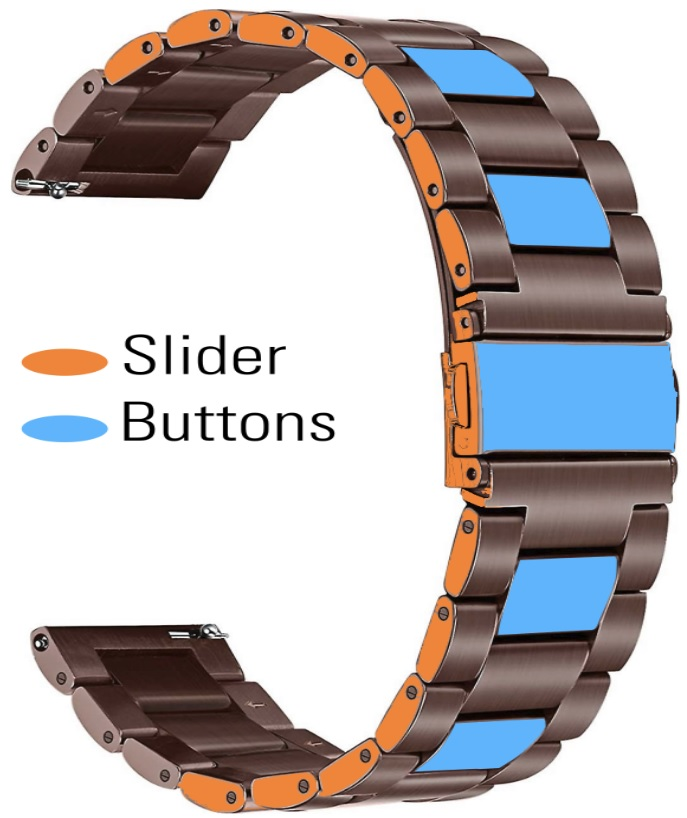
\includegraphics[scale=.35]{assets/Strap_initial_idea.jpg}
	\caption{Konzept }
	\label{fig:Initial_Idea}
\end{figure}

Dieses Konzept sieht vor, ähnlich wie in einem metallenen Armband die Drucksensoren auf die einzelnen Glieder des Armbandes zu verteilen und als Buttons zu verwenden. Zudem soll die Seite des Armbandes als Slider via Berührungssensoren Wischbewegungen unterstützen.\\	
Man entschied sich mit dem Konzept fortzufahren. Die nächste Frage, welche Beantwortung finden musste war, ob ein bereits existierendes Uhrenarmband für den Prototypen modifiziert werden soll oder ob man selbst von Grund auf einen Prototyp entwickeln möchte?\\
Es wurde sich festgelegt, nicht bereits existierende Armbänder bzw. Uhrenarmbänder zu modifizieren, sondern ein Prototyp von Grund auf zu entwerfen. Insbesondere für inkrementelle Änderungen oder schnelles Testen von Ideen bietet dieses Vorgehen mehr Flexibilität innerhalb des Prozesses. Unter anderen war diese Entscheidung auch dadurch begründet, den finanziellen Faktor möglichst gering zu halten, sowie dass keiner der Gruppenmitglieder adäquates Werkzeug zur Bearbeitung von Leder besitzt oder Metall besitzt. Das Armband der Galaxy Watch zu Verwenden wurde auch schnell ausgeschlossen.\\
Im nächsten Schritt wurden die Zuständigkeiten der Bearbeitung der einzelnen Projektbereiche festgelegt und das restliche Hardwareprototyping unter Sektion \ref{sec:Hardwareprototyping} wurde von Florian übernommen.\\

\newpage

Abbildung \ref{fig:concept_layout} wurde

\begin{figure}[h]
	\centering
	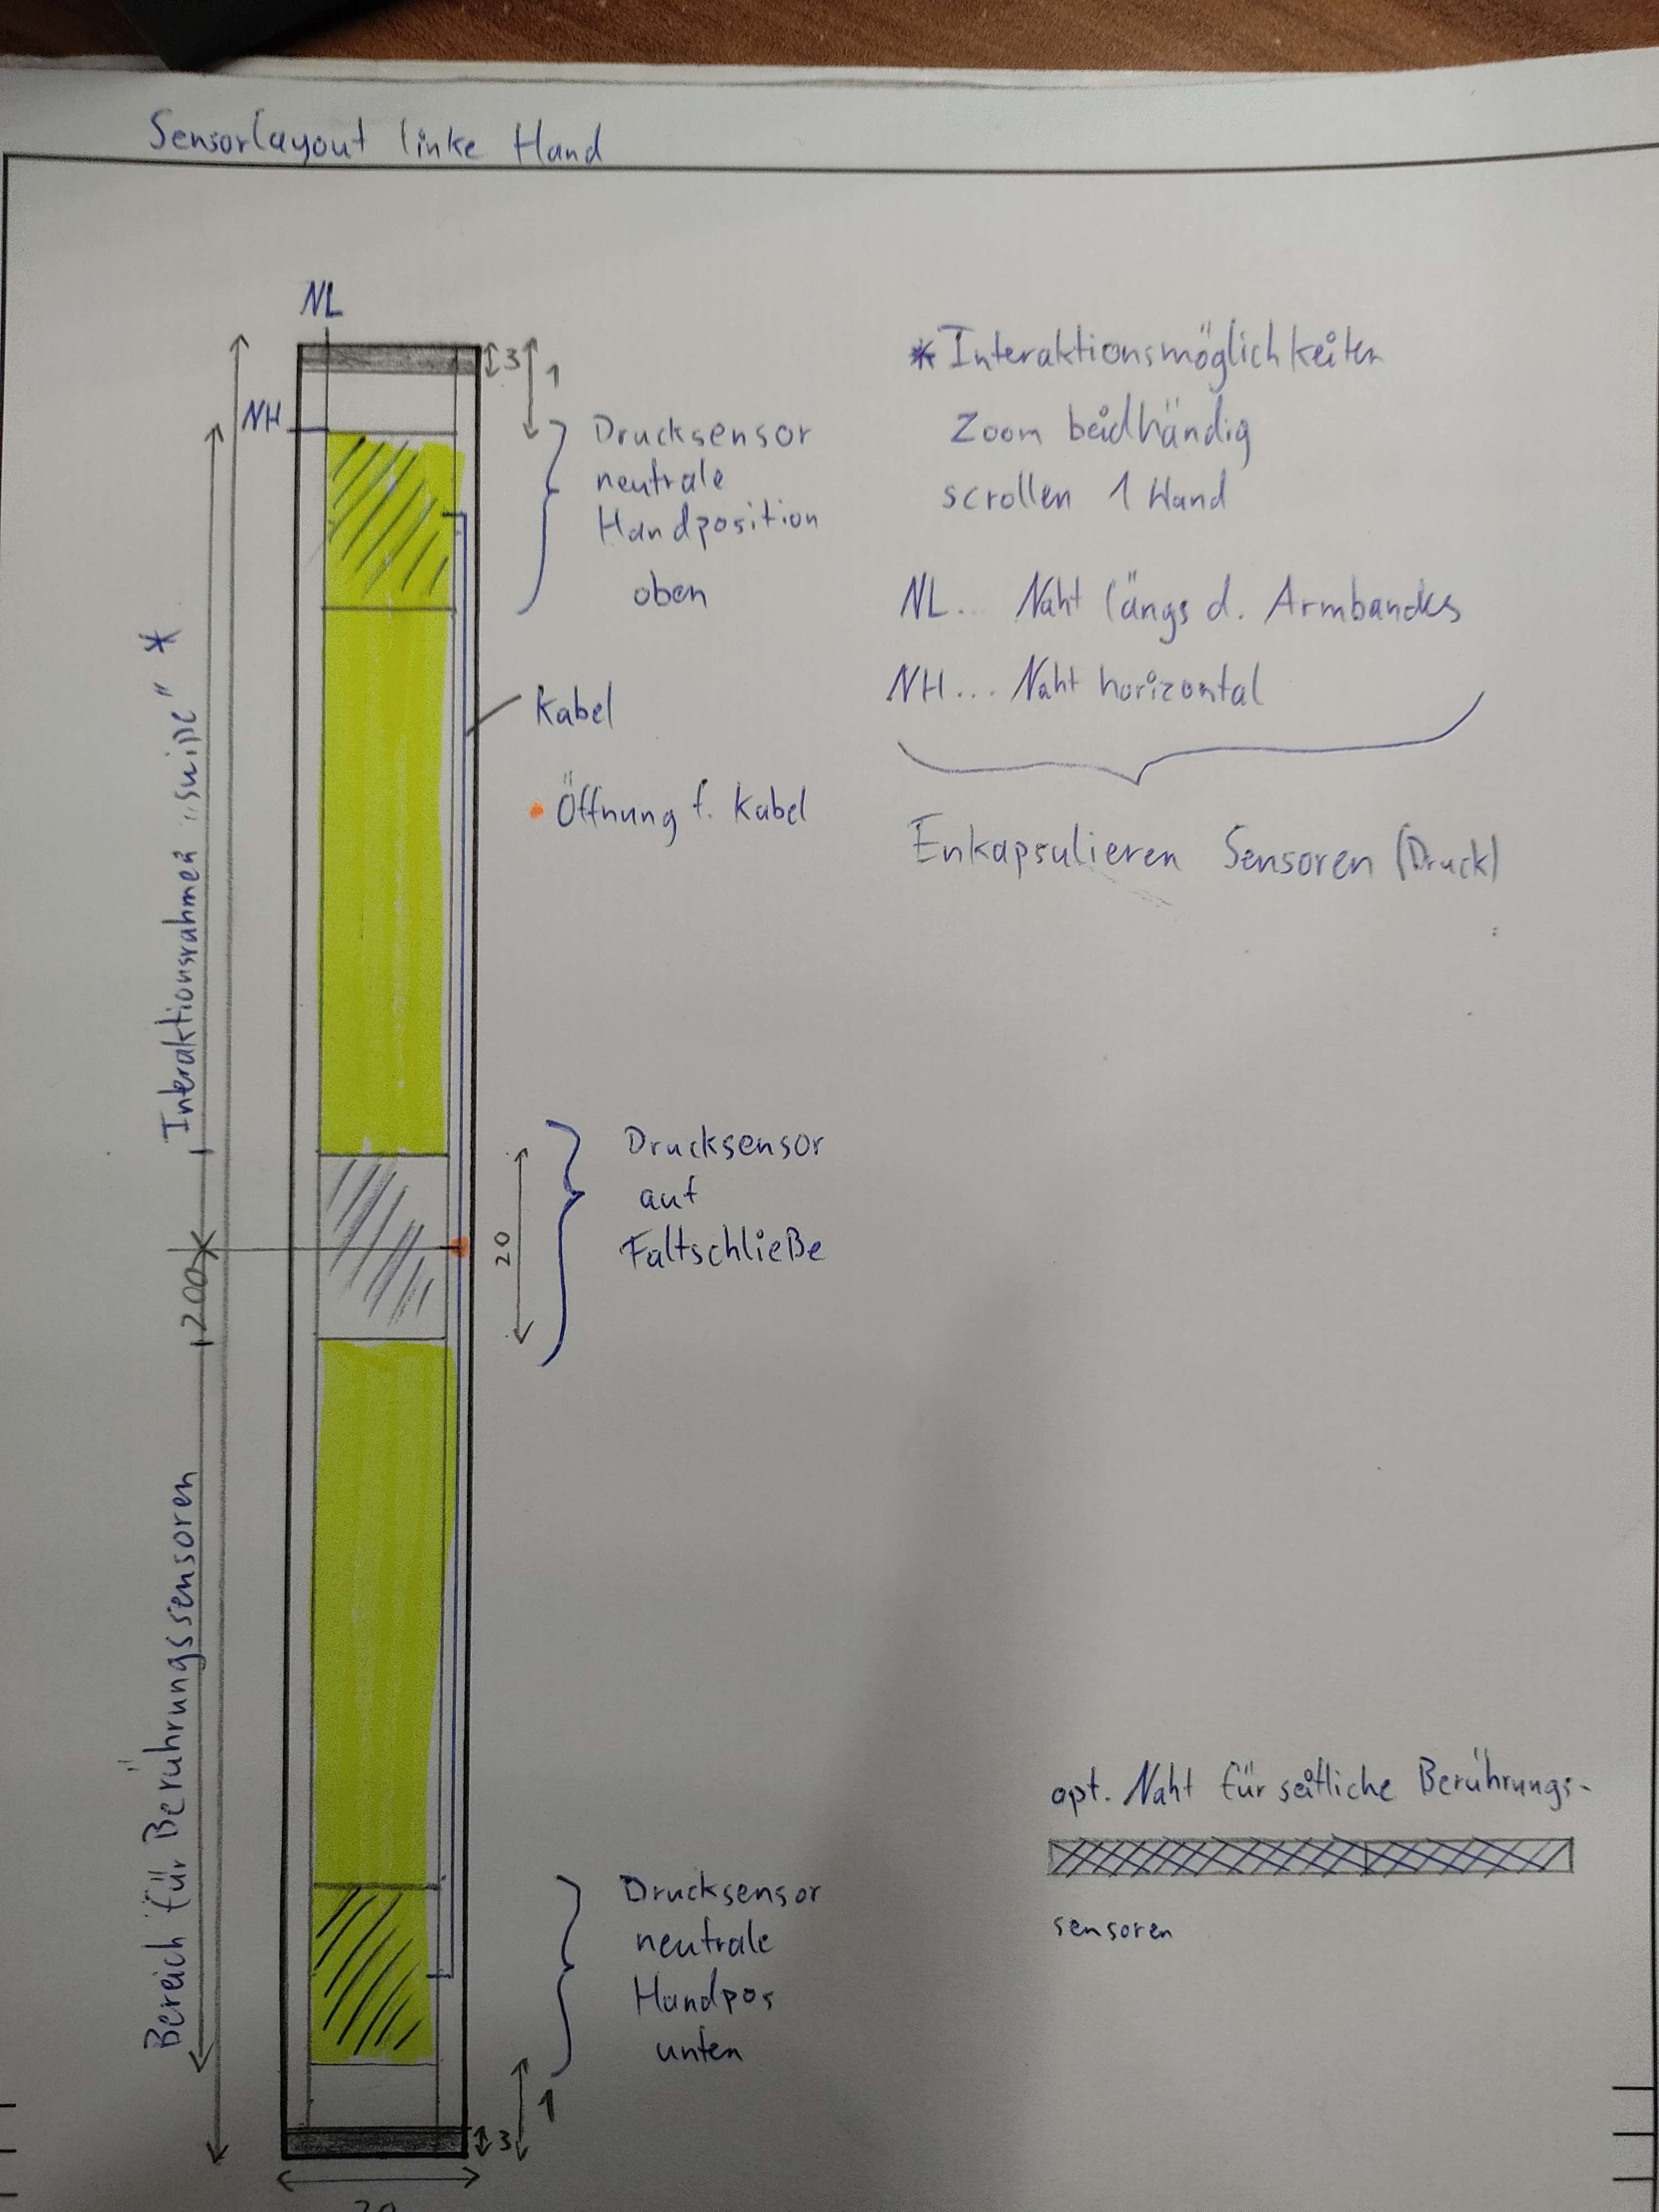
\includegraphics[scale=.1]{assets/Design_drawing.jpg}
	\caption{Konzept Layout}
	\label{fig:concept_layout}
\end{figure}

\newpage

Es musste nun geklärt werden welche Materialien zur Entwicklung infrage kämen. Die Anforderungen an das Material waren: Der Stoff des Armbandes darf nichtleitend sein und muss sich nähen lassen, zudem sollte er verformbar sein, um Bewegungen der Uhr am Armband standzuhalten, jedoch nur minimal dehnbar und natürlich den Formfaktor umsetzen können. Nach Initialrecherche für infrage kommende Materialien wurde schnell klar, Mantelstoffe wie (gekochte) Wolle mit variablen Verhältnis von Naturfaser zu Kunstfaser (oft 80\% Schurwolle, 20\% Polyamid) gibt es in unterschiedlichen Stärken, wäre gut für die Umsetzung. Preislich jedoch sprengte das den Rahmen als Substitution bat sich Filz an, Kompromisse müssen damit im Erscheinungsbild in Kauf genommen werden, jedoch erfüllt Filz alle Anforderungen und bieten den großen Vorteil die Schnittkante des Stoffes muss wie bei der Wolle nicht nachbehandelt werden. Somit 

\newpage




\begin{figure}[h]
	\centering
	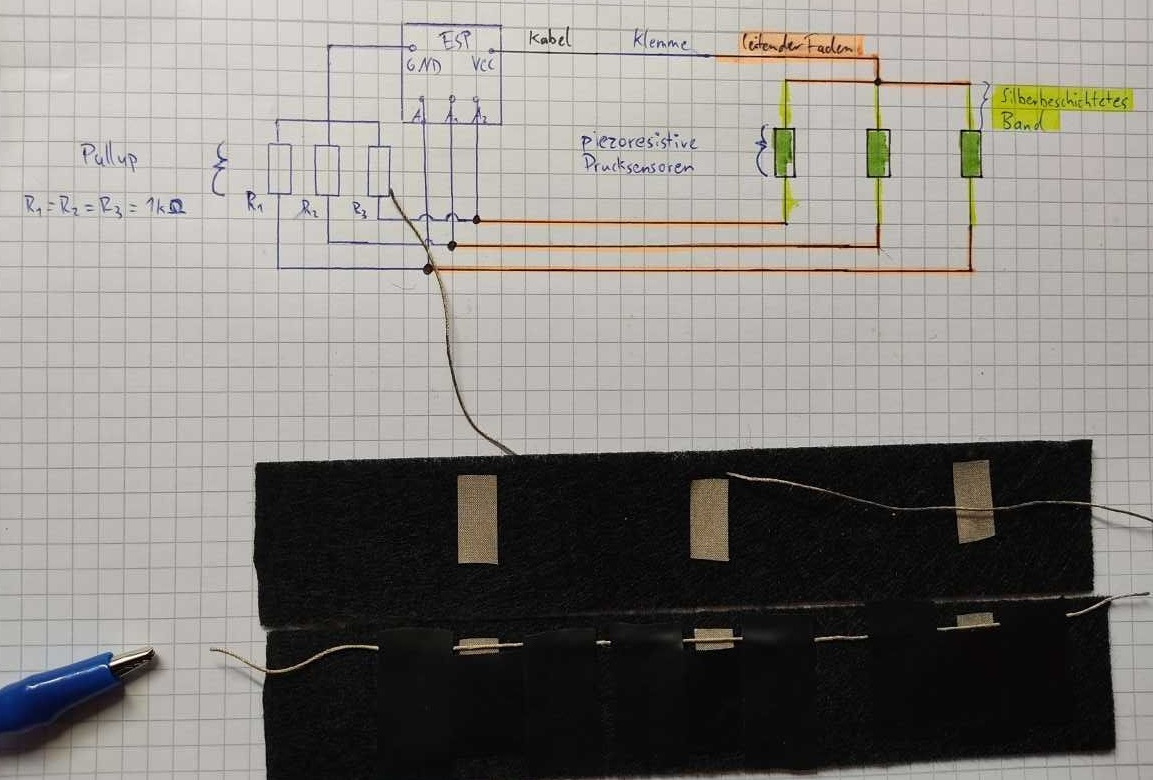
\includegraphics[scale=.5]{assets/Prototyp.jpg}
	\caption{ayaa}
	\label{fig:Initial_drawing}
\end{figure}










\begin{figure}[h]
	\begin{subfigure}[c]{0.33\textwidth}
		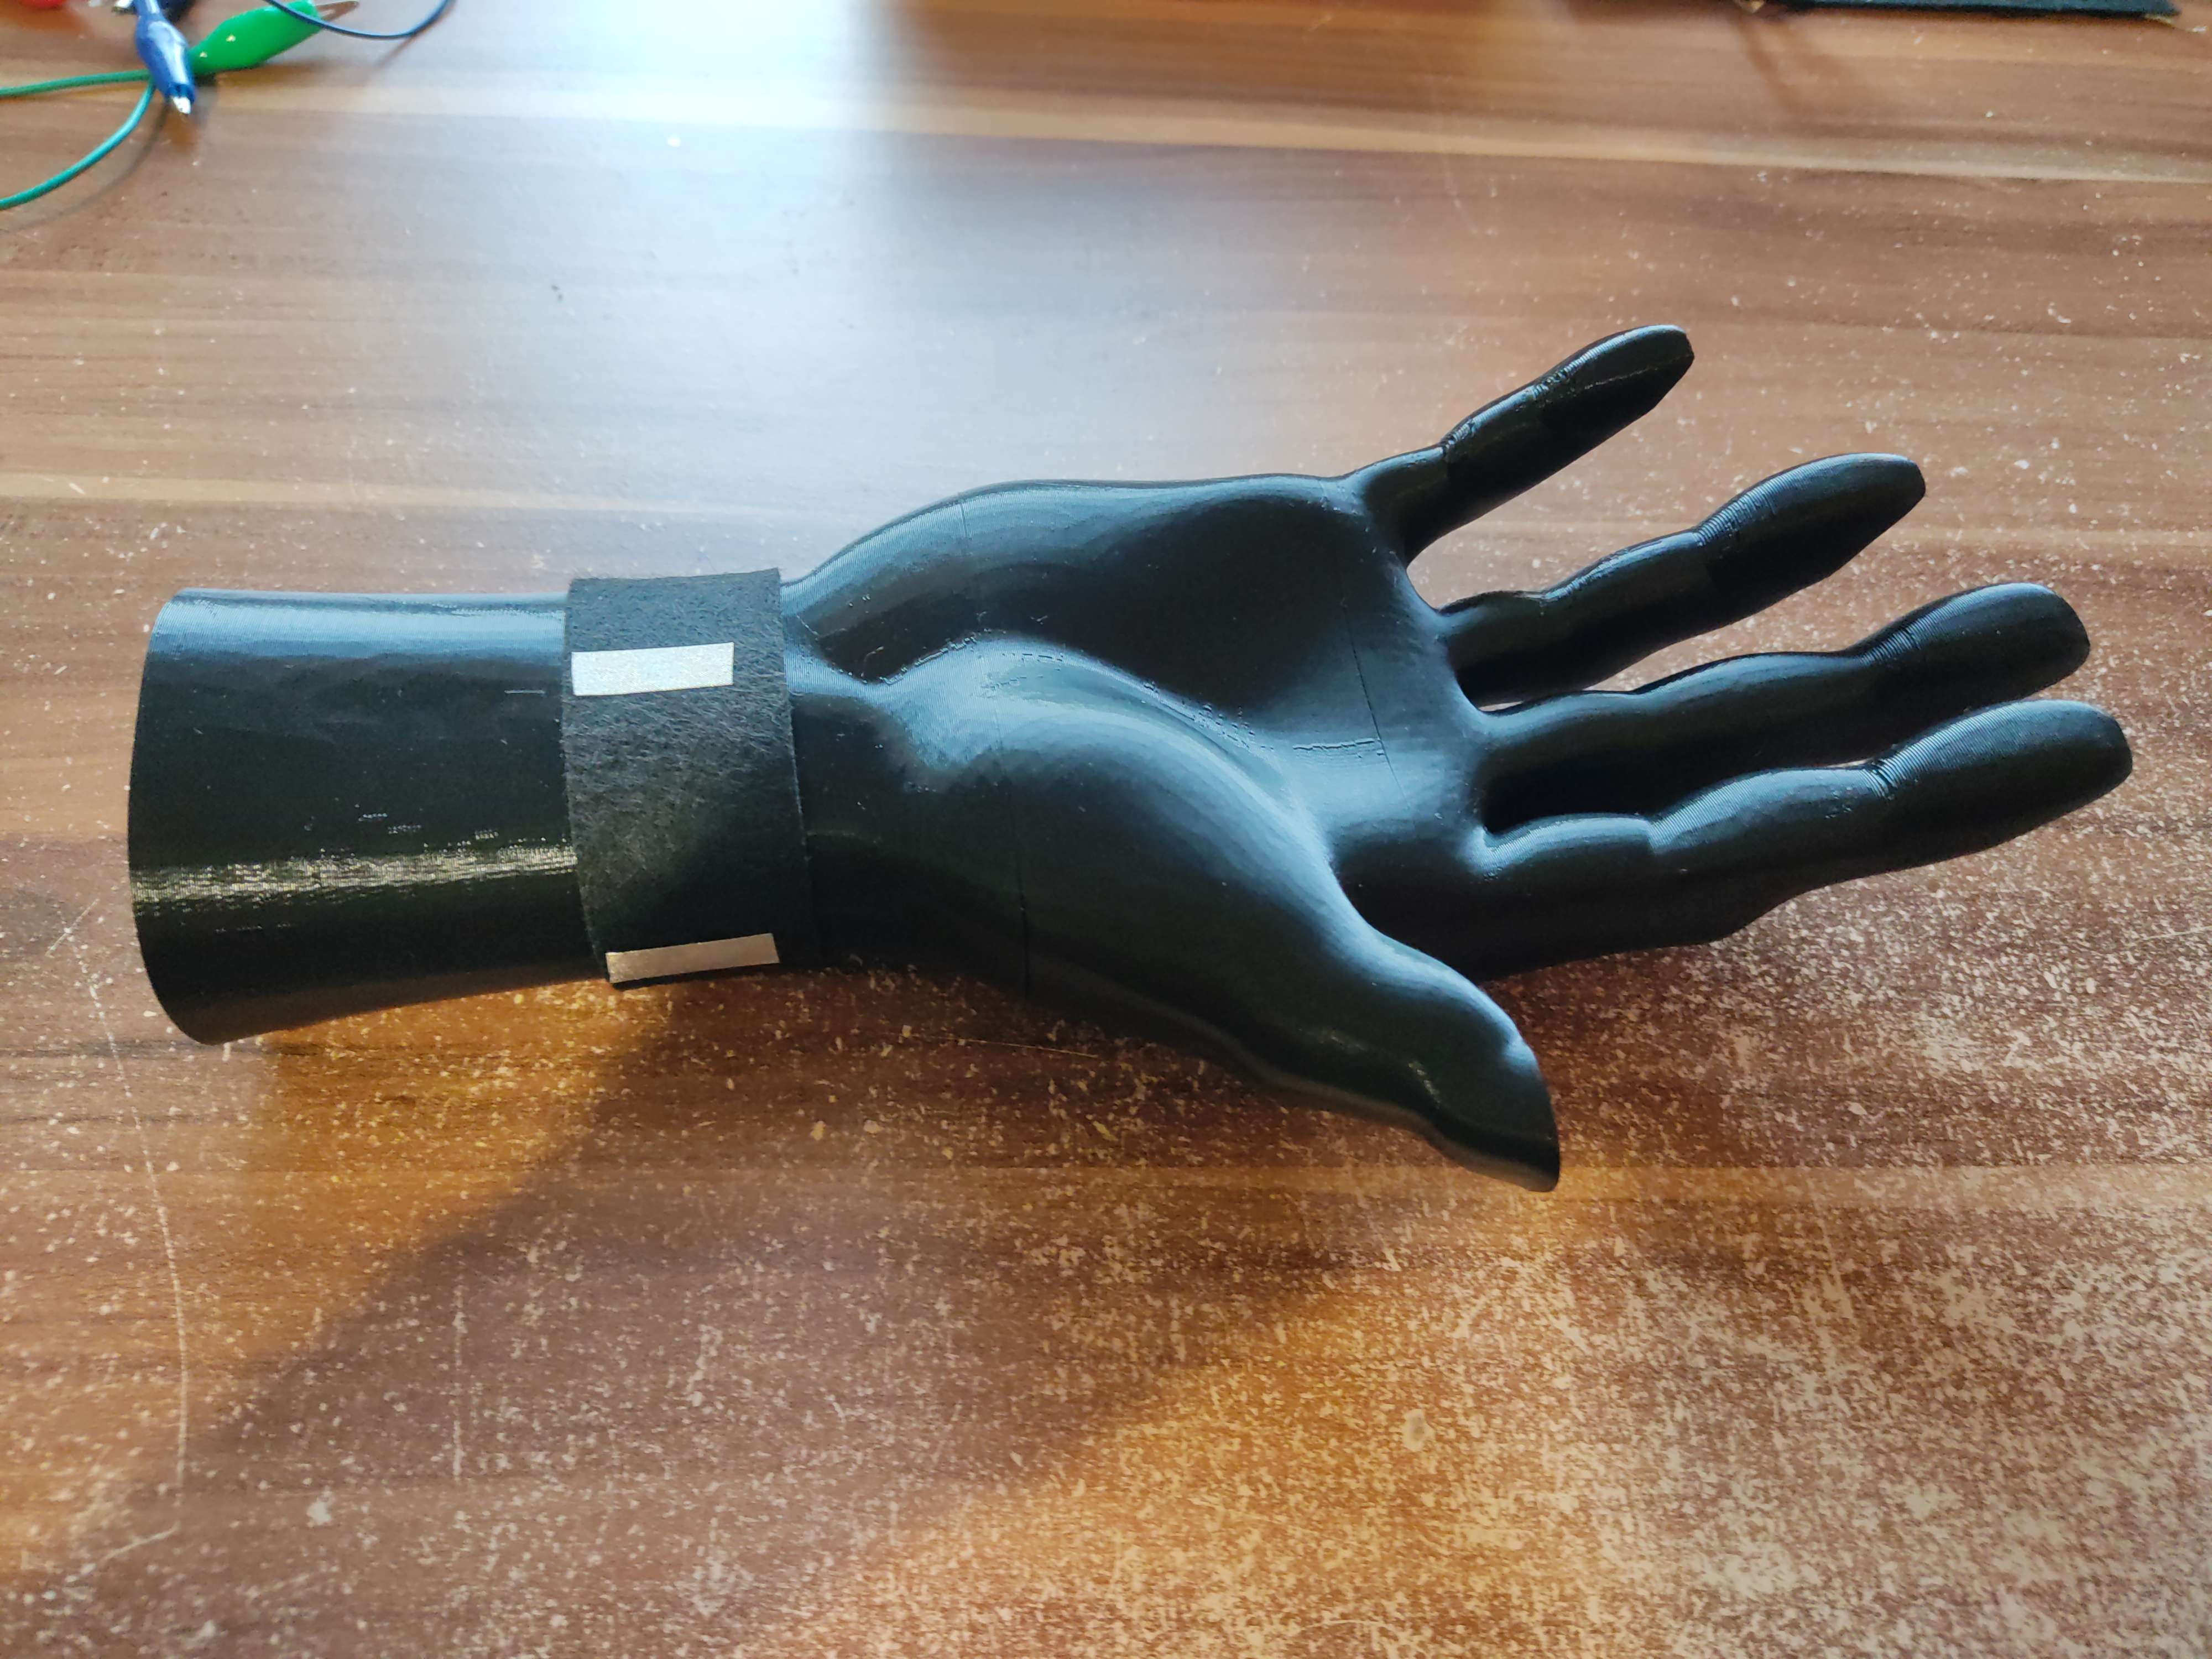
\includegraphics[scale=.037]{assets/Strap_fitting_wires.jpg}
		\caption{Platzierung für Bohrung}
		\label{fig:Initial_drawing}
	\end{subfigure}
	\begin{subfigure}[c]{0.33\textwidth}
		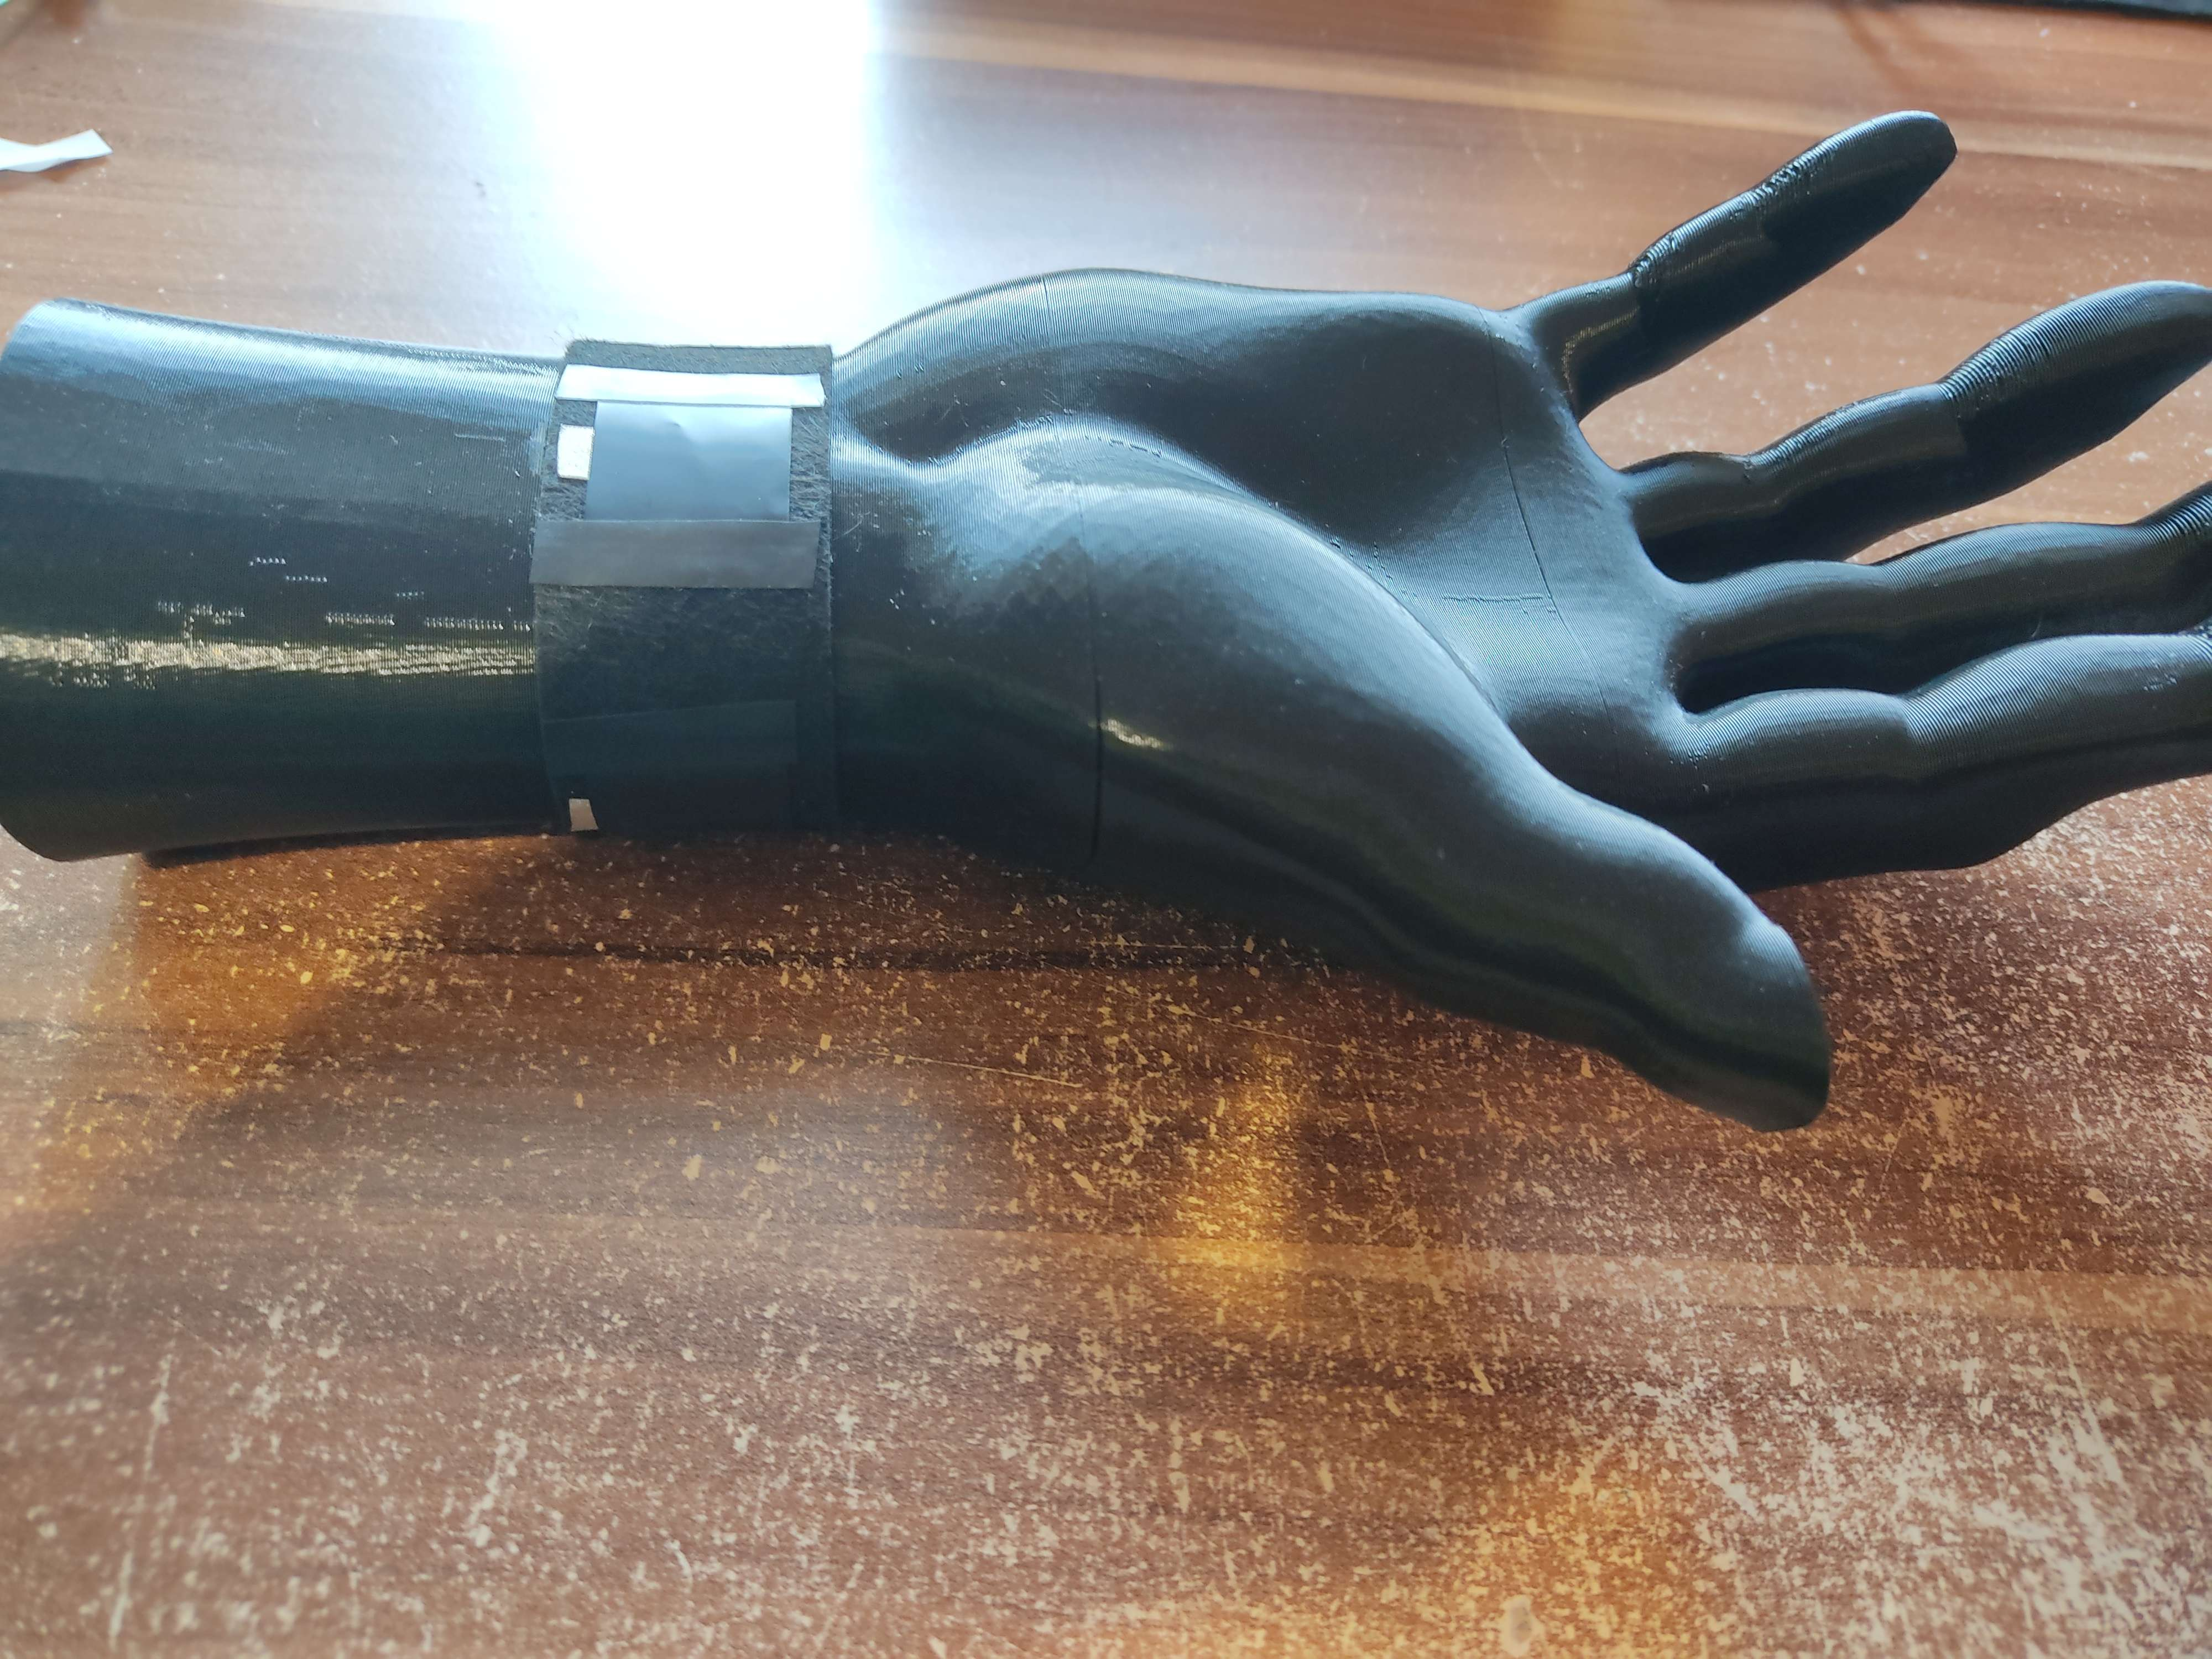
\includegraphics[scale=.037]{assets/Strap_fitting_sensors.jpg}
		\subcaption{Sensorplatzierung}
		\label{fig:Initial_drawing}
	\end{subfigure}
		\begin{subfigure}[c]{0.33\textwidth}
		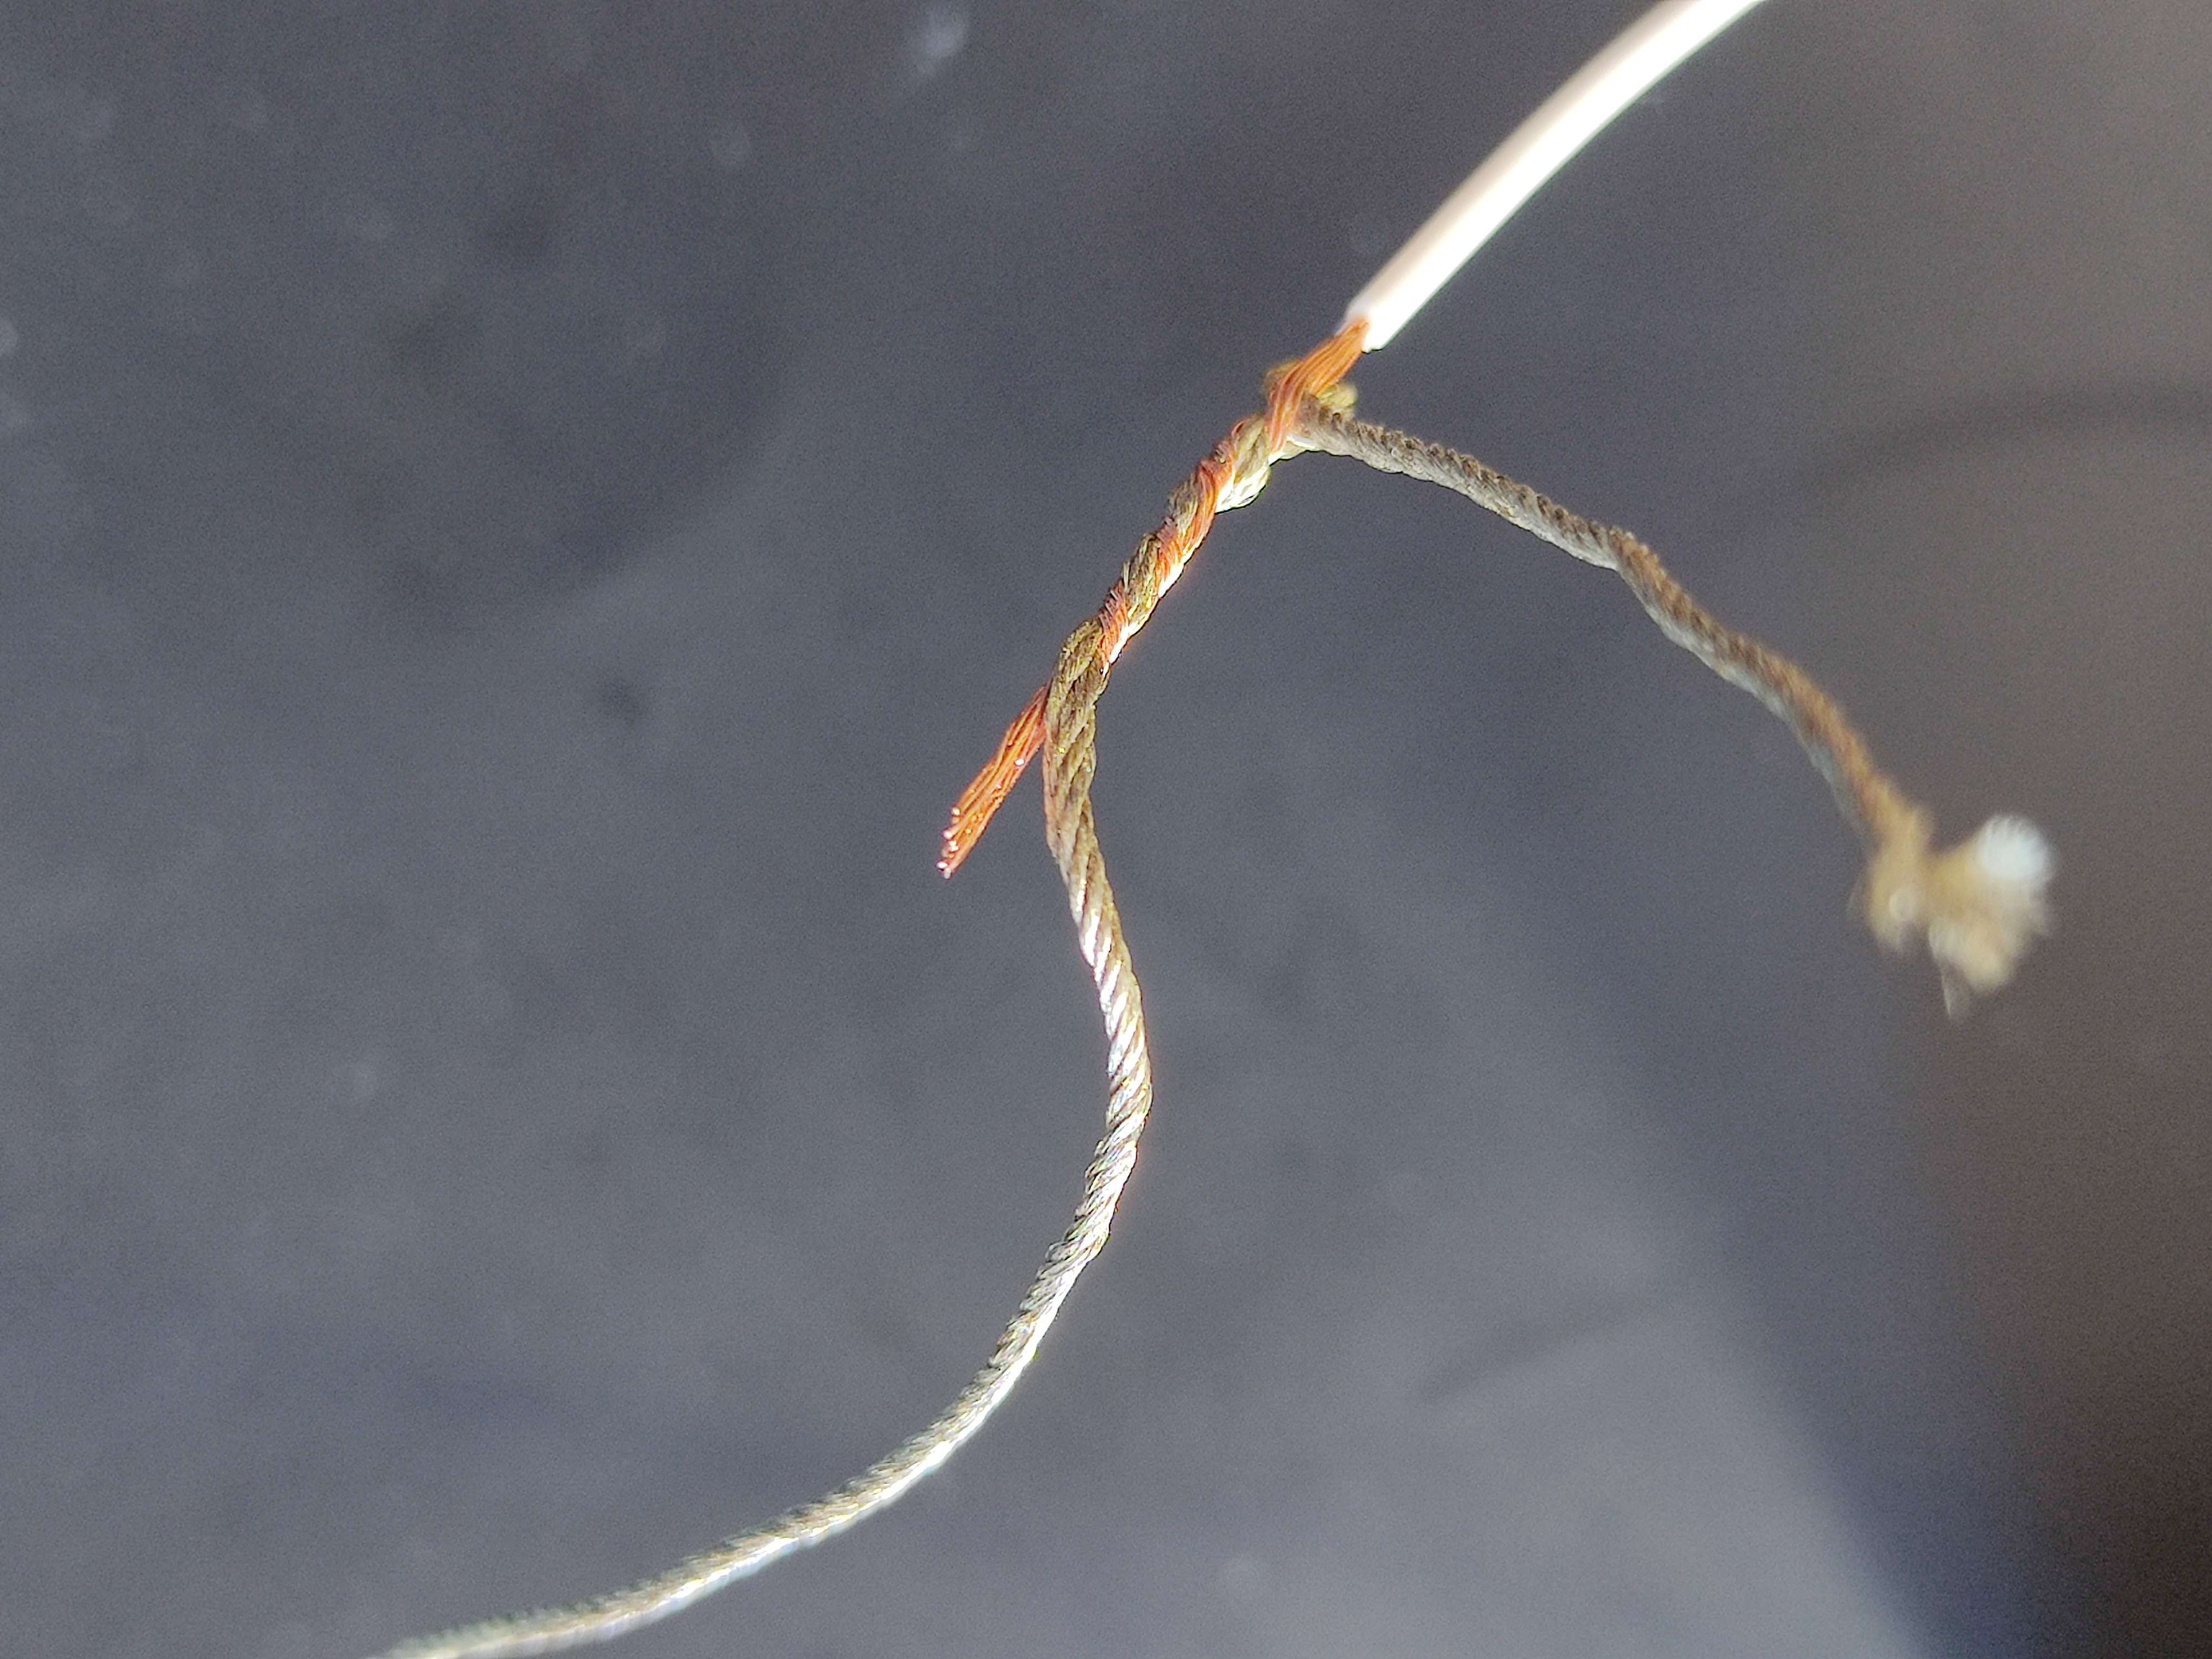
\includegraphics[scale=.037]{assets/Connection_thread_wire.jpg}
		\subcaption{Verbindung Garn und Draht}
		\label{fig:Initial_drawing}
	\end{subfigure}
	\caption{Fitting bracelet to hand}
\end{figure}
ayaya
\begin{figure}[h]
	\begin{subfigure}[c]{0.33\textwidth}
		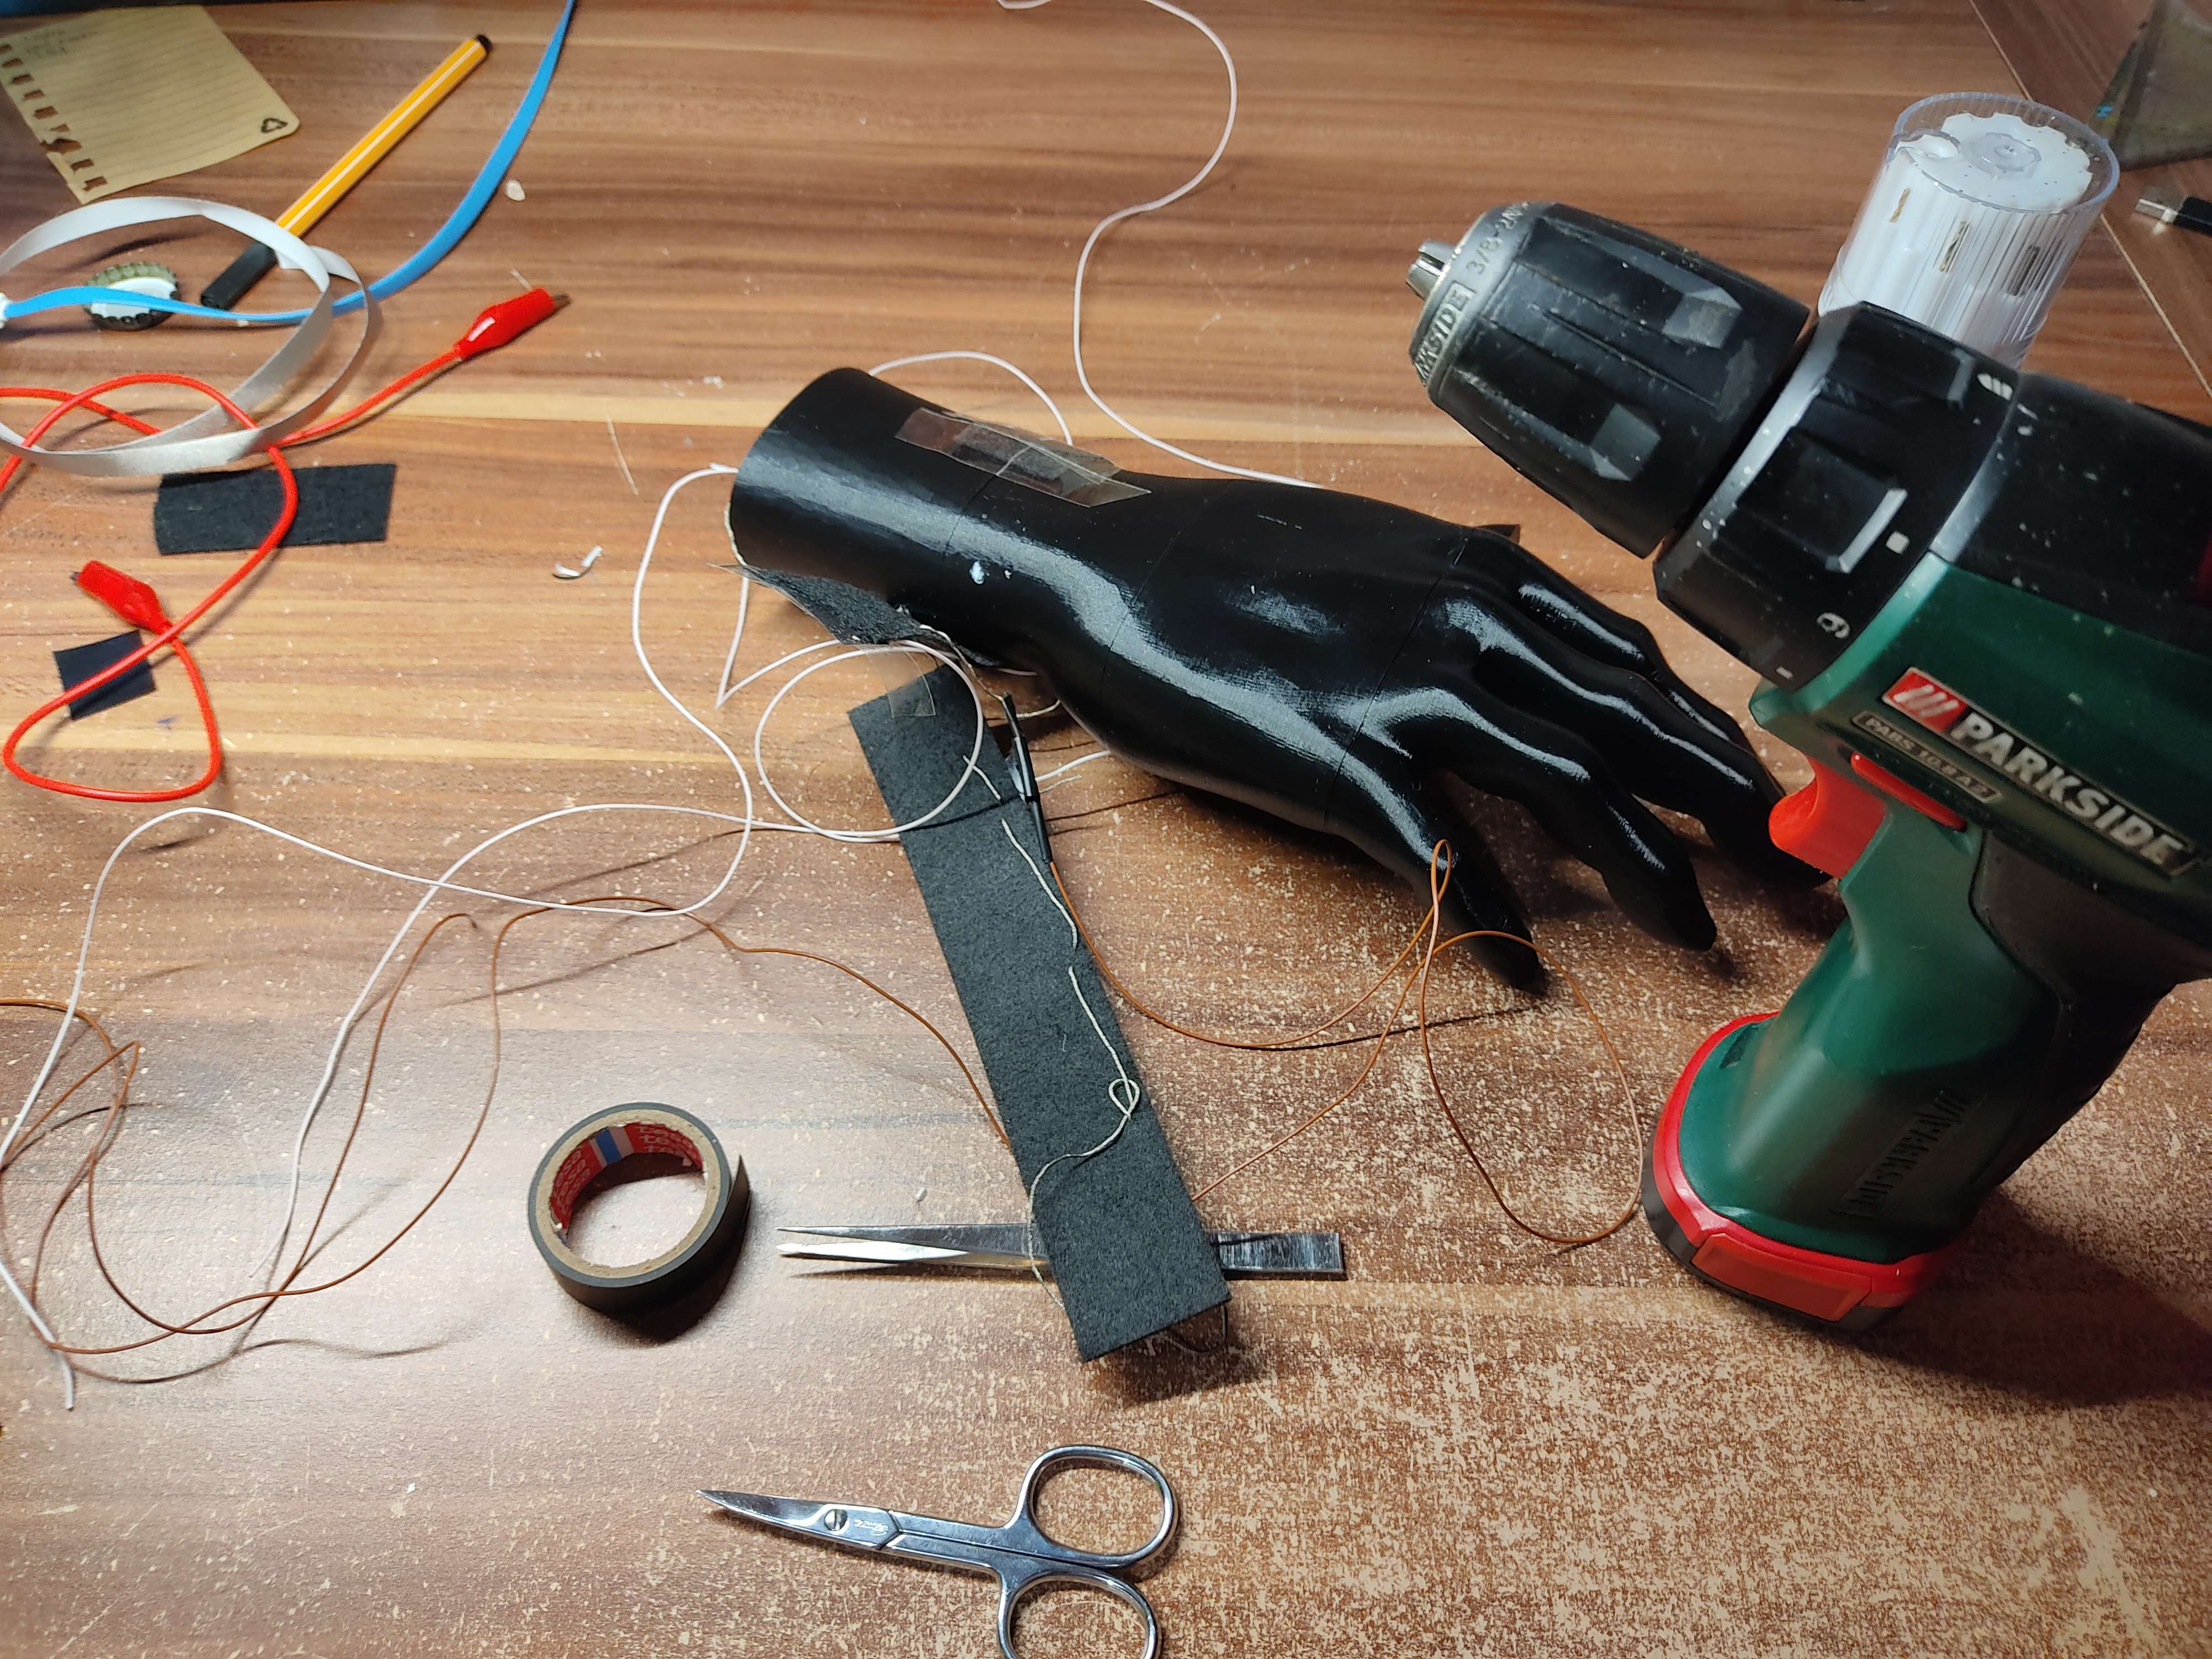
\includegraphics[scale=.037]{assets/Drill_markers.jpg}
		\caption{Löcher bohren}
		\label{fig:Initial_drawing}
	\end{subfigure}
	\begin{subfigure}[c]{0.33\textwidth}
		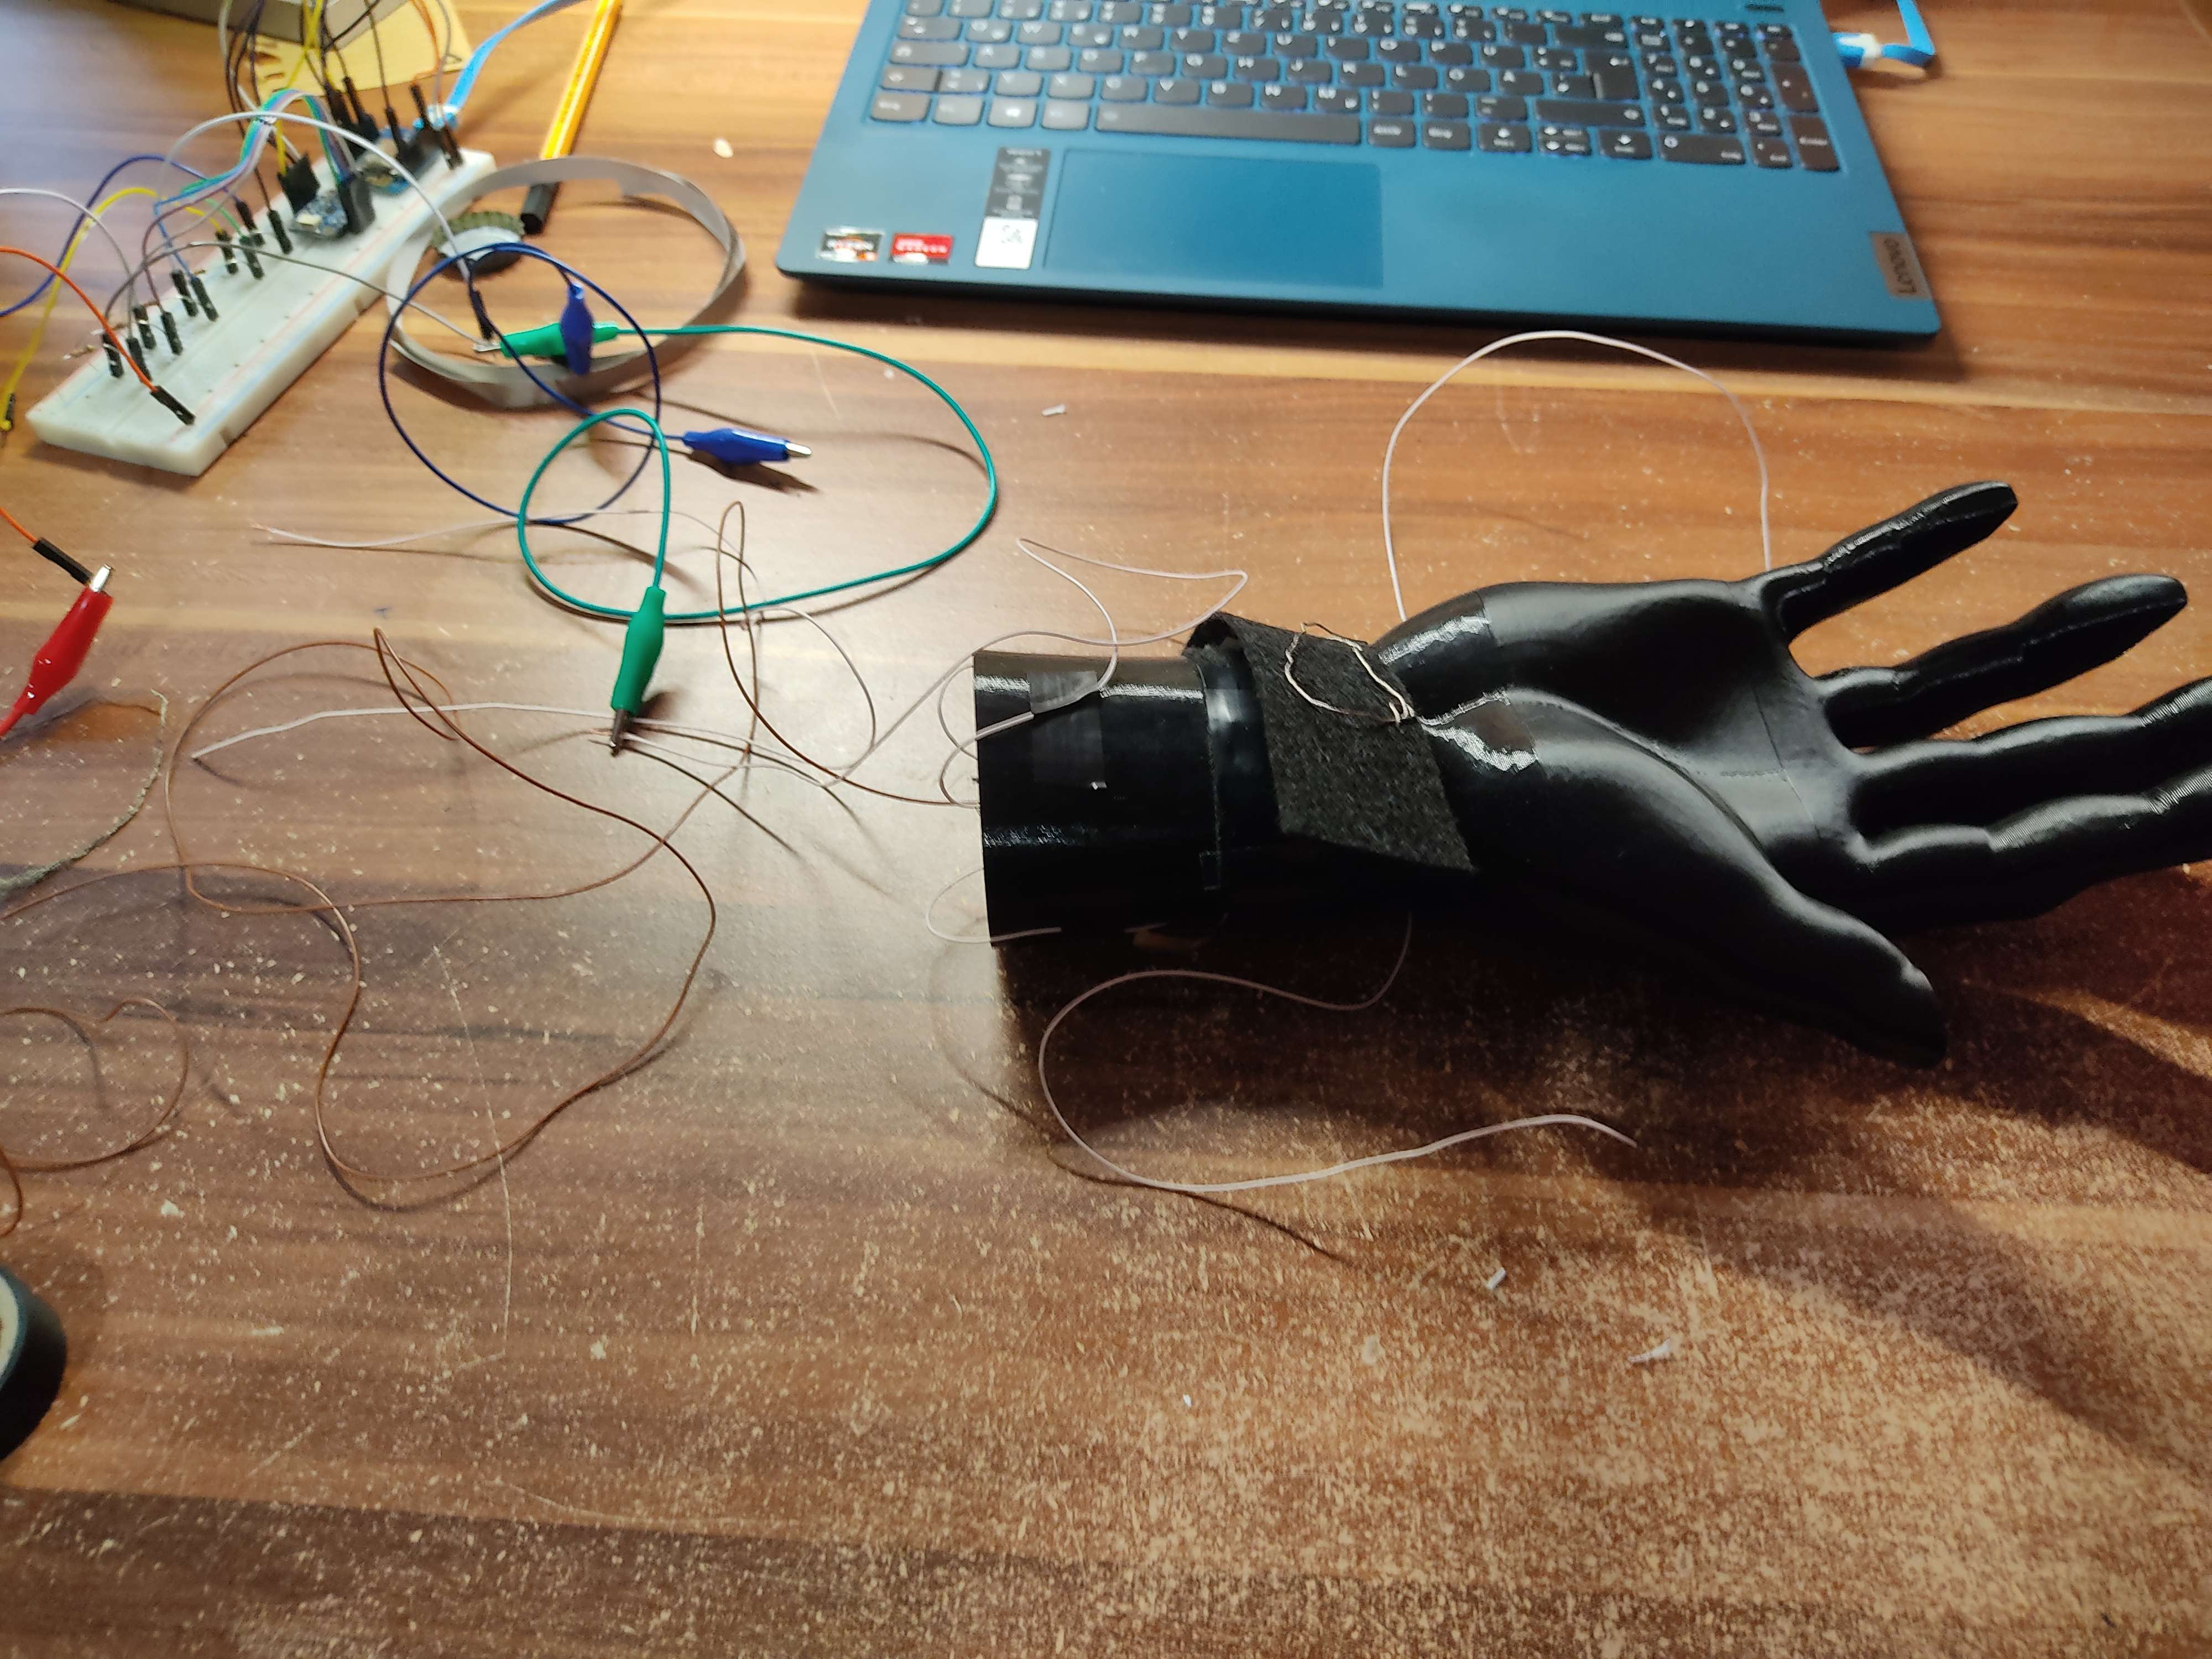
\includegraphics[scale=.037]{assets/Testing_before_finalizing.jpg}
		\subcaption{Testen ob Kurzschluss}
		\label{fig:Initial_drawing}
	\end{subfigure}
		\begin{subfigure}[c]{0.33\textwidth}
		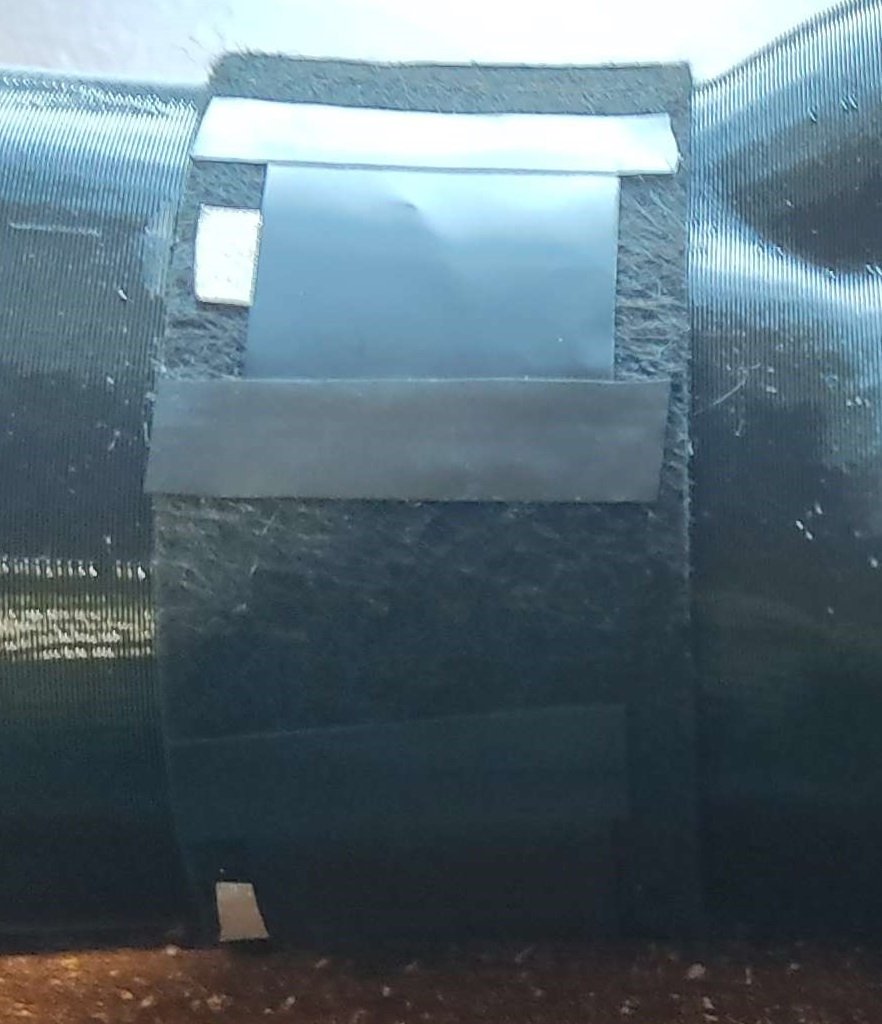
\includegraphics[scale=.037]{assets/crop_sensor_fitting.jpg}
		\subcaption{Finaler Prototyp}
		\label{fig:Initial_drawing}
	\end{subfigure}
	\caption{Fitting bracelet to hand}
\end{figure}






Nach Anforderungsanalyse an das Armband haben sich 3 Schwerpunkte ergeben. Welches Material ist für das Armband geeignet? Welche Sensoren sollen Verwendung finden und welche Eingabemodalitäten sind sinnvoll, also wo sollen diese Sensoren platziert werden.


\subsection{Arduino}


\begin{enumerate}
	\item{Erhalte Sensoreingabe}	
	\item{cut out noise}
	\item{remap ads overreadings}
	\item{filter out unintentional inputdata}
	\item{send tcp}
\end{enumerate}

\subsection{final thing}

\subsection{Designprozess}

WeMos D1 Mini ESP8266, erweitert um ein Adafruit ADS1015 für bis zu 5 single Channel Analog input 3-5 pull ups
@TODO bild

ESP Analogwerte $\in \{0,...,1023\}$
ADS Analogwerted $\in \{0,...,1100\}$ $\to $ map 

ADS Analogwerte sind teilweise zufällig 2\^16 groß, ohne Eingabe -> Noise rausschneiden. Armbänder werden für gewöhnlich nah am Körper getragen, um unintentionelles Auslösen der Sensoren zu verhindern, werden Eingabewerte der Sensoren zwar registriert, aber nicht behandelt, dies wird durch ein Treshholding der Eingabestärke also einen erhöhten Druck auf den Sensor erreicht. Idealerweise ist das für weitere Anwendungen mit dem Gyroskop des MEMS der Smartwatch zu verbinden um beispielsweise nur Werte zu betrachten, wenn der Arm in Wagerechter Position sich befindet und dann Eingabe über das Armband erfolgt. 


\subsection{finale Eingabemodalitäten}

\section{Interfaces und Integration}

\subsection{Protokolle}

\subsection{Systemintegration}

\section{Smartwatch-App Prototyp}

\subsection{Ideenfindung}

Zunächst war für unseren Prototyp keine Smartwatch-App vorgesehen. Auch, da uns dafür die nötige Hardware gefehlt hat und eine Beschaffung nicht in unserem Budget liegen würde. Erst im Gespräch mit unseren Betreuern haben wir eine Samsung Galaxy Gear s3 für die Einbindung in unseren Prototypen in Aussicht gestellt bekommen. Daraufhin mussten wir uns zunächst die Frage stellen, welchen Zweck die Uhr in unserem Produktprototyp erfüllen sollte. Nach einigem Überlegen haben wir uns dazu entschieden, die Smartwatch als zentrales Element unseres Prototyps zu sehen und die auf der Uhr gewählten Anwendungen durch eine Visualisierung und eine Steuerung durch das Armband zu ergänzen. Somit sollte auf der Uhr eine App laufen, die eine Auswahl aus verschiedenen Anwendungen erlaubt. 

\subsection{Lo-Fi-Prototyp}

Als Start in die Umsetzung haben wir zunächst einen Lo-Fi-Prototyp skizziert, um die App, die Sichten und die Navigation zu entwickeln. Dabei ist diese Skizze entstanden (siehe Abbildung \ref{fig:Smatwatch_Prototyp}).

\begin{figure}[h]
	\centering
	\includegraphics[scale=.35]{assets/lo_fi_prototyp.jpeg}
	\caption{Lo-Fi-Prototyp}
	\label{fig:Smatwatch_Prototyp}
\end{figure}

In diesem Lo-Fi-Prototyp waren zunächst drei Sichten definiert. Die Erste sollte ein Home Bildschirm sein. Dies soll ein Default Case sein, in welchem die Smartwatch-App gestartet wird, aber noch keine Anwendung ausgewählt ist. Durch eine Swipe Geste nach rechts oder links, hier durch die Pfeile gekennzeichnet, sollte zwischen den verschiedenen Sichten gewechselt werden können. Die anderen zwei Sichten sollen symbolisieren, dass hier eine Anwendung hinterlegt ist. 

\subsection{Tizen}

Nachdem wir nun also einen ersten theoretischen Prototyp entwickelt hatten, ging es nun an die praktische Implementierung. Dazu mussten wir uns zunächst in die Grundlagen der Tizen Entwicklung einarbeiten und ein neues Projekt aufsetzen. Dabei haben wir uns an dem Watch+Strap Tizen App Projekt der TU Dresden [Quelle: https://github.com/imldresden/WatchStrap-tizen-app] orientiert. 
Nach der Einarbeitung und dem Aufsetzen des neuen Projekts galt es zunächst, die Grundfunktionalitäten der Smartwatch sicherzustellen. Dazu müssten Klassen wie der lowBatterryCheck oder auch die Button-Events für “back” und “main” implementiert werden. 

\subsection{Erstfassung der Smartwatch-App}

Als die Grundfunktionalitäten schließlich implementiert waren, konnten wir uns an die Umsetzung unserer App machen. Dazu haben wir zunächst eine einzelne index.html Seite implementiert, die sich in mehrere sections gegliedert hat. Durch einen Swipe oder durch die Basal Rotation wurde die sectionChange Methode aufgerufen, welche wiederum die nächste section sichtbar gemacht hat. 


\begin{figure}[h]
	\centering
	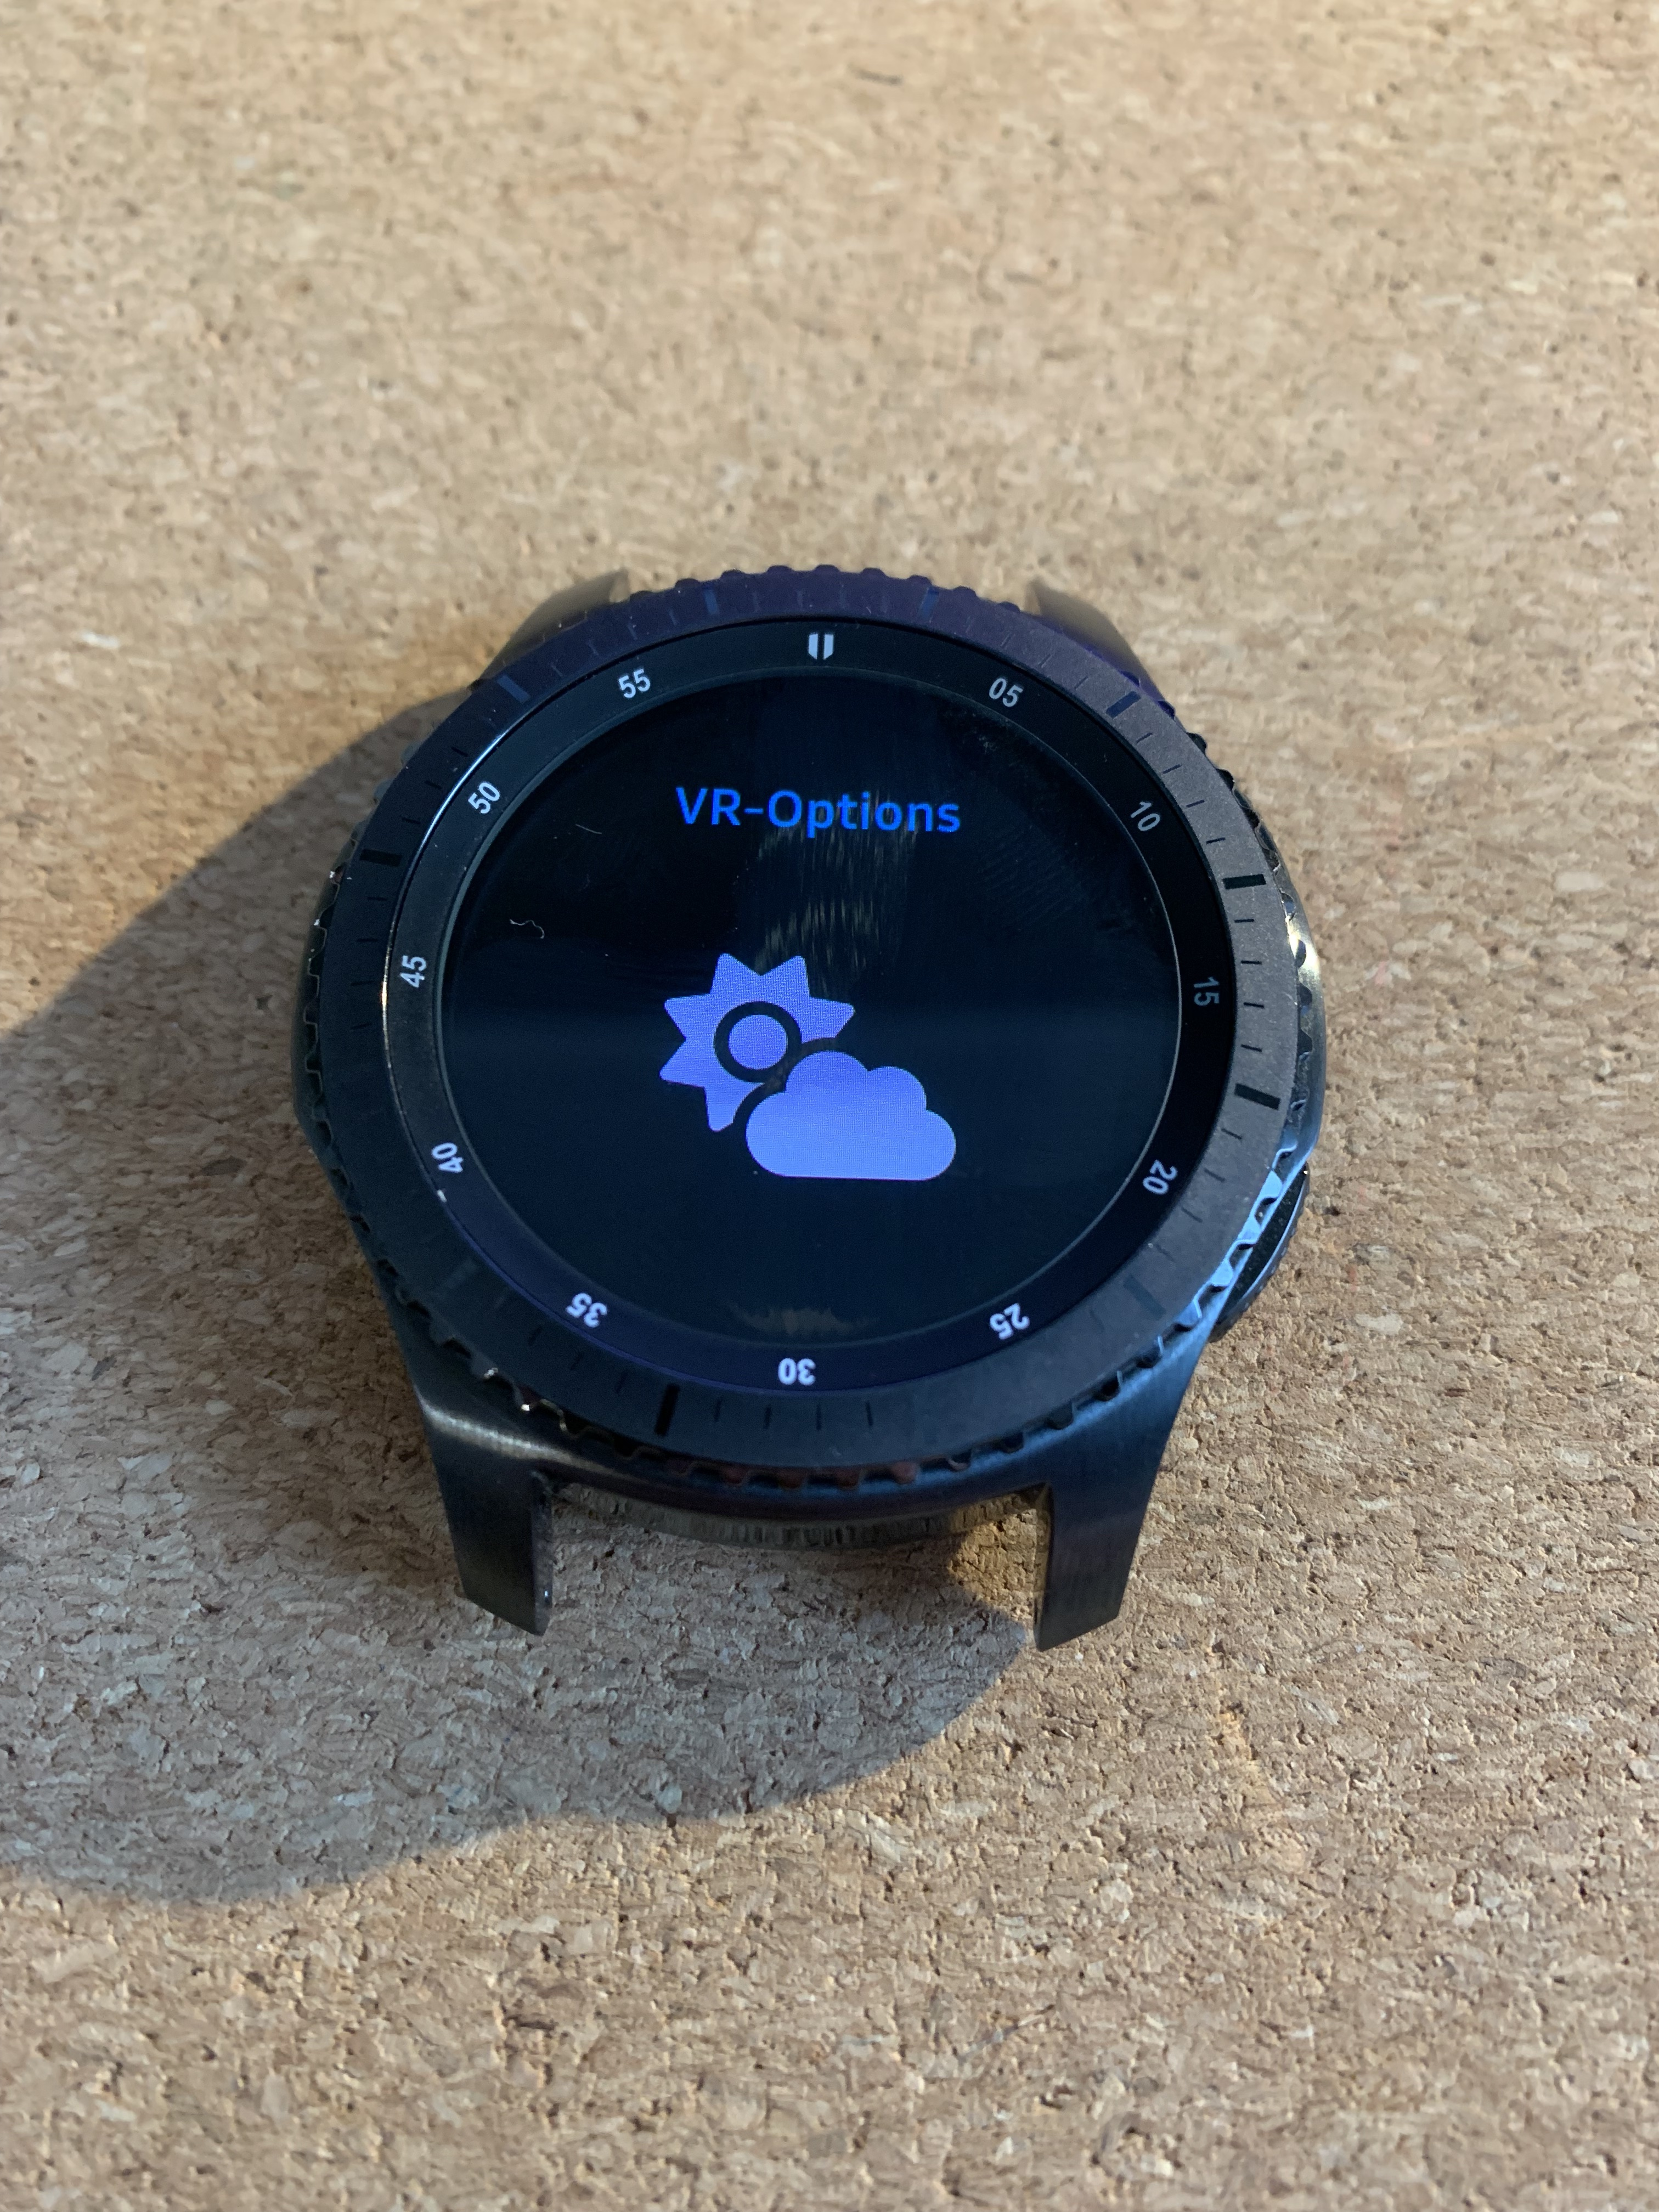
\includegraphics[scale=.35]{assets/smartwatch_app_erstversion.jpg}
	\caption{Weather Anwendung in früher Version}
	\label{fig:app_erstversion}
\end{figure}

Die Abbildung zeigt beispielhaft eine ausgewählte section, die mit dem Wetter-Icon versehen ist. Das Produkt dieses Abschnittes war eine Tizen-App, die durch Swipegesten oder die Basal Rotation gesteuert durch die sections Home, Weather und Documents bewegt werden konnte. 

\subsection{Websockets}

Als nächster Schritt stand nun die Verbindung zu unserem Unity-Projekt an. Dabei mussten wir zunächst eine geeignete Technologie für unsere Netzwerkübertragung finden. Der erste Versuch war, eine HTTP-Massage zu verschicken. Dies ließ sich zwar aufseiten der Smartwatch-App als Client gut implementieren, dennoch stellte es sich als umständlich heraus, auf Unityseite einen HTTP-Server zu implementieren. Deswegen entschieden wir uns, die Technologie Websockets umzustellen. Nun können folgende Nachrichten von der Smartwatch-App an die Unity-Anwendung verschickt werden: 

\begin{enumerate}
	\item{“0” - Home section / zurück auf Home section}	
	\item{“1” - weather section}
	\item{“2” - graph section}
	\item{“3” - documents section}
	\item{“a1” - weather Anwendung gestartet}
	\item{“a2” - graph Anwendung gestartet}
	\item{“a3” - documents Anwendung gestartet}
	\item{“cw” - Clockwise Rotation}
	\item{“ccw” - counterClockwise Rotation}
\end{enumerate}

Auf Seiten von Unity gibt es einen mit WebSocketSharp erstellten Websocket-Server. Dieser kann die Nachrichten empfangen und in der Methode StateChange.SetAppState() zur Weiterverarbeitung in Unity zur Verfügung stellen. 

\subsection{Zweitfassung der Smartwatch-App}

Nachdem die Websocket-Kommunikation implementiert war, kam noch der Wunsch auf, auch innerhalb der einzelnen Anwendungen die Basal-Rotation zur Steuerung der Visualisierung nutzen zu können. Deswegen braucht es eine Trennung zwischen der Anwendungsauswahl, die ebenfalls über die Basal-Rotation möglich ist, und der Anwendung selbst. Aus diesem Grund haben wir einen Button auf das jeweilige App-Auswahlfeld gemacht, der eine HTML-Unterseite aufruft, die eigene Scripte lädt und so eine Trennung von der Auswahl einer App und dem "in einer App sein" ermöglicht. 

\begin{figure}[h]
	\centering
	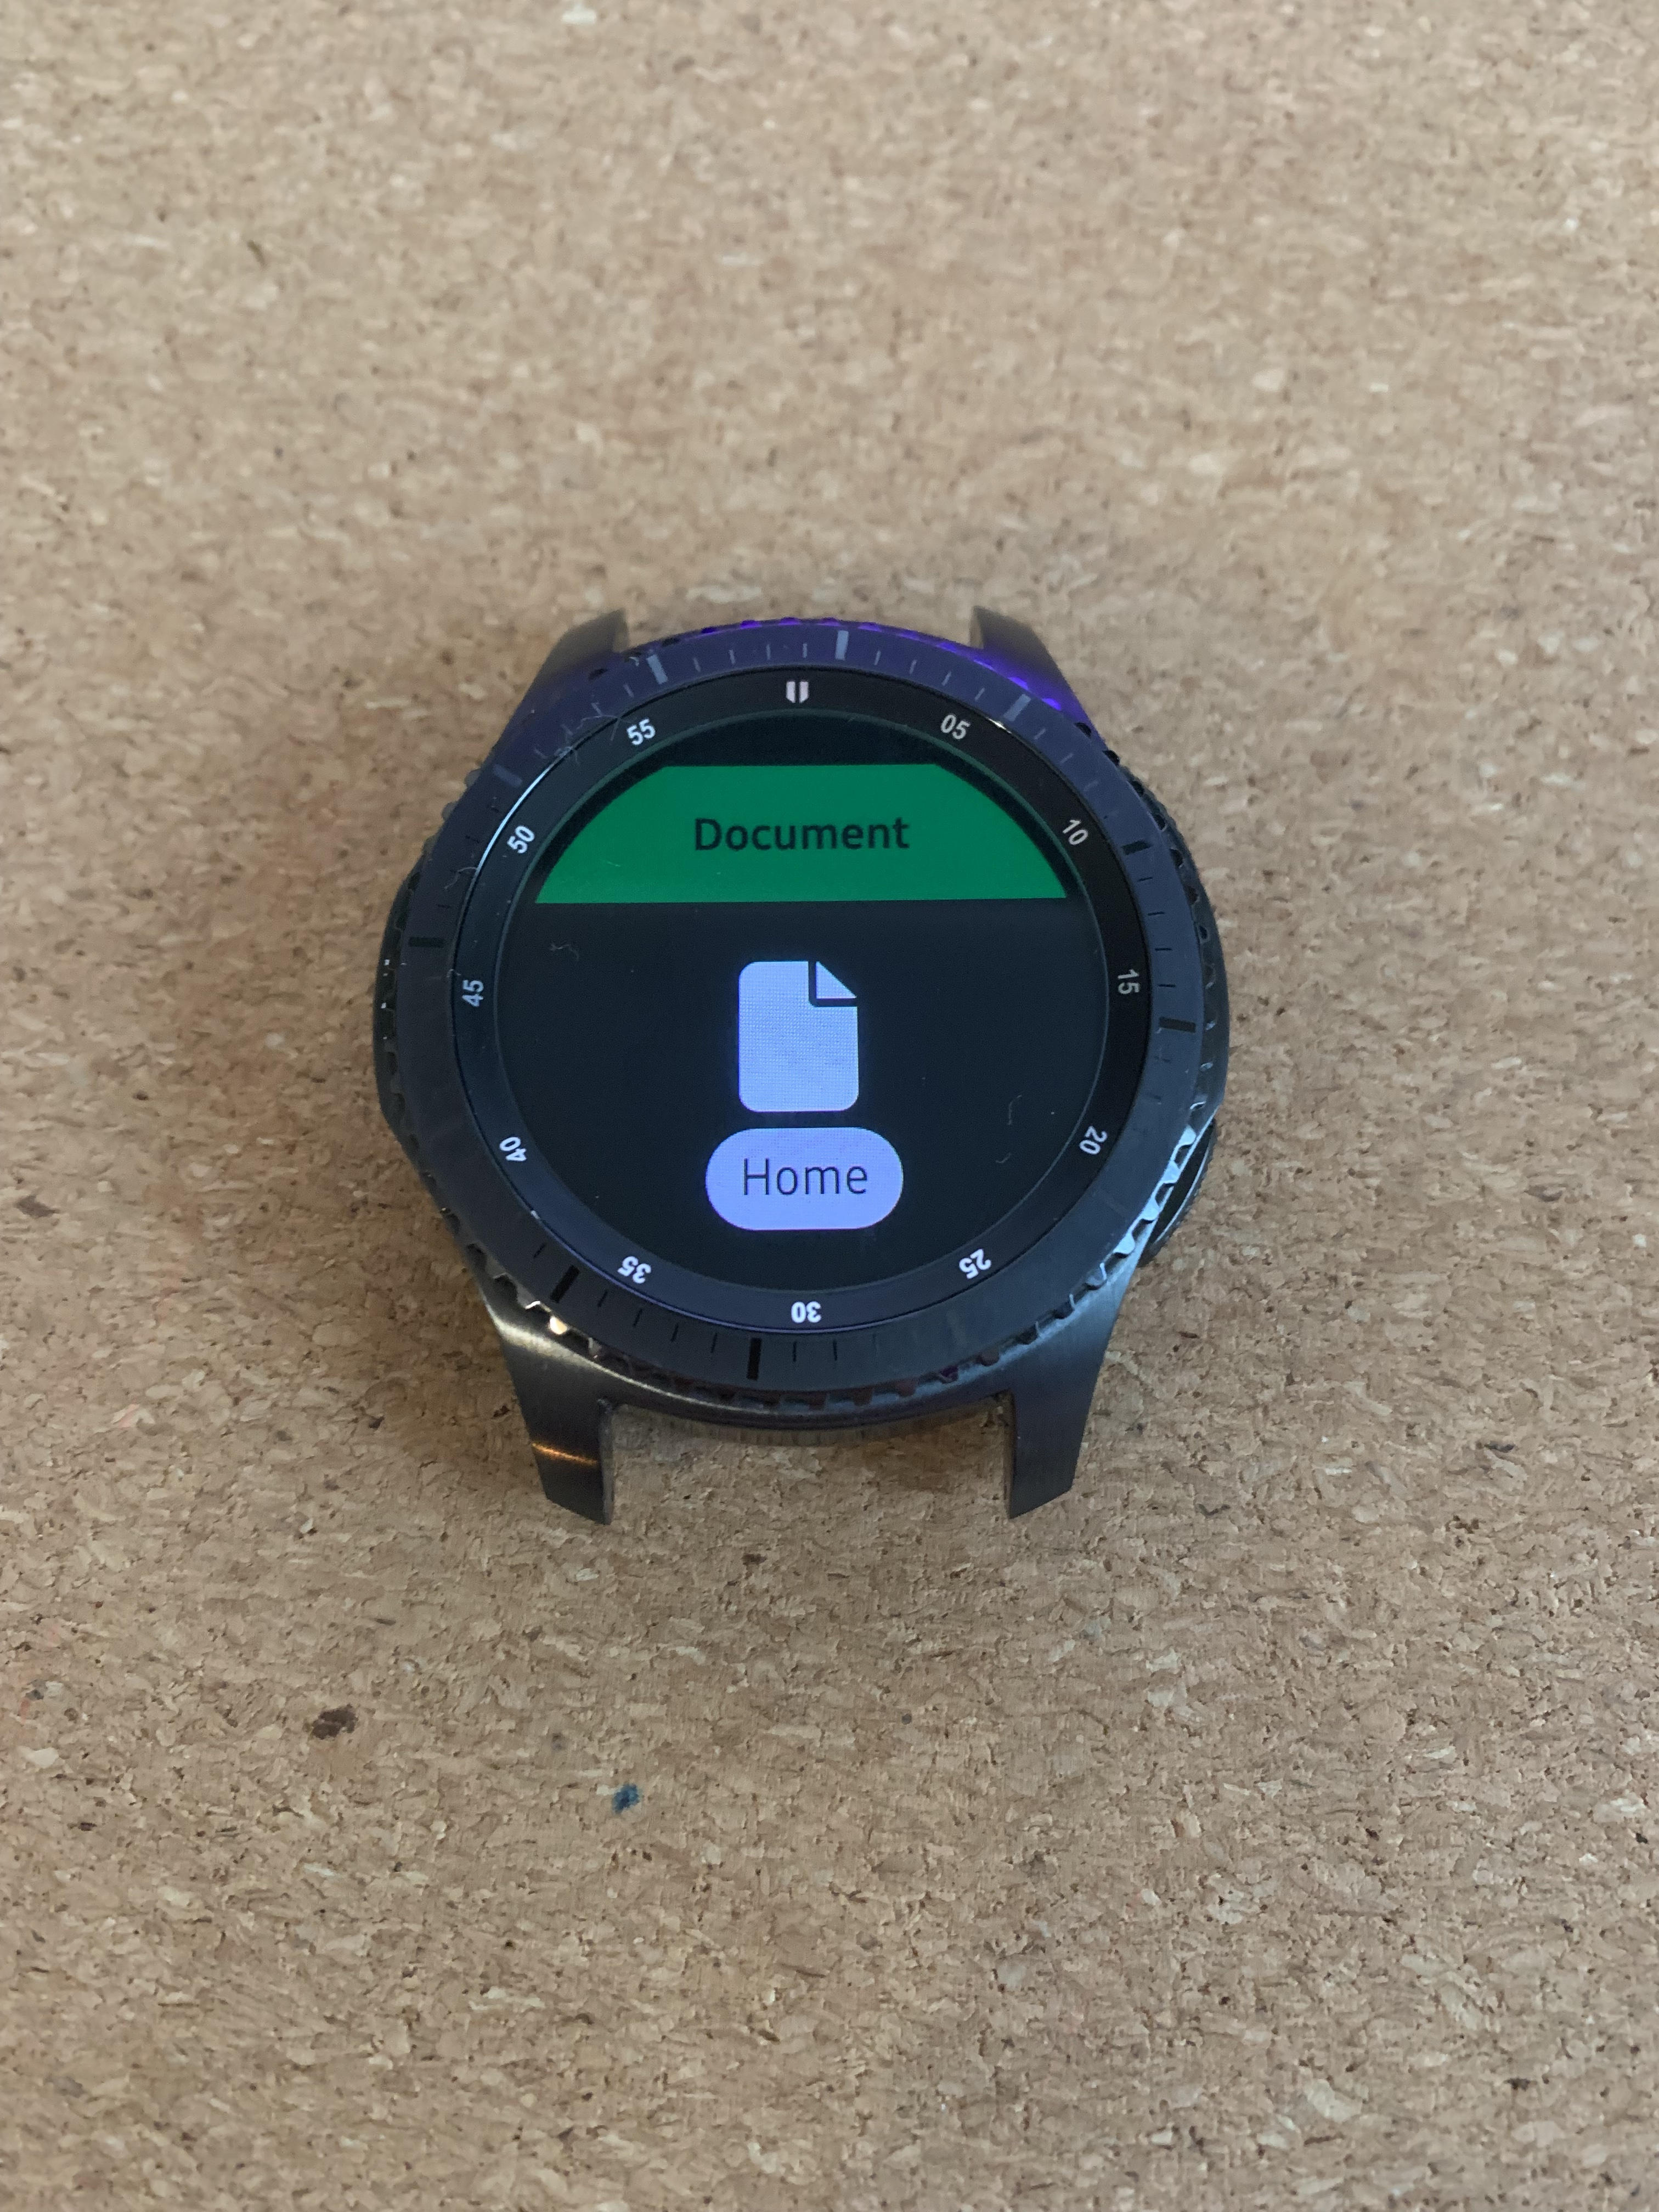
\includegraphics[scale=.35]{assets/smartwatch_app_zweitversion.jpg}
	\caption{Finale Documents Anwendung}
	\label{fig:app_zweitversion}
\end{figure}

Wie in der Abbildung zu erkennen, haben wir die Anwendungsseite auch farblich an die Visualisierung angelehnt gestaltet, um so auch visuell noch eine Verbindung zwischen der Smartwatch-App und der Unitiy Visualisierung zu schaffen. 

\subsection{Systemintegration}

Die Smartwatch-App gliedert sich in das Gesamtprojekt als Element zur Anwendungsauswahl und zur Steuerung ein. So kann über die App eine Unter-Anwendung Weather, Graph oder Documents ausgewählt und durch einen Button-Klick gestartet werden. Durch die Basal-Rotation können bestimmte Elemente der Visualisierung darüber hinaus auch gesteuert werden. Außerdem kann über den Home Button eine Anwendung wieder geschlossen werden. 


\end{document}